
%        نمونه پایان‌نامه آماده شده با استفاده از کلاس Razi-Thesis، نگارش 0.1
% 	     امین روشنی، دانشگاه رازی، دانشکده علوم، گروه آمار
%        این نسخه، بر اساس نسخه‌ 0.4 از کلاس Tabriz_Thesis آقای وحید دامن‌افشان آماده شده است. http://damanafshan.tk        
%---------------------------------------------------------------------------------------------
%        اگر قصد نوشتن پروژه کارشناسی را دارید، در خط زیر به جای msc، کلمه bsc و اگر قصد نوشتن پروژه دکترا
%        را دارید، کلمه phd را قرار دهید. کلیه تنظیمات لازم، به طور خودکار، اعمال می‌شود.
\documentclass[phd]{Razi-Thesis}

% مشخصات دانشجو و پایان‌نامه، سوگندنامه، برگ اصالت و مالکیت اثر، تشکر و قدردانی را در فایلهای faTitle و enTitle وارد نمایید.

%       فایل commands.tex را مطالعه کنید؛ چون دستورات مربوط به فراخوانی بسته زی‌پرشین 
%       و دیگر بسته‌ها و ... در این فایل قرار دارد و بهتر است که با نحوه استفاده از آنها آشنا شوید.
% در این فایل، دستورها و تنظیمات مورد نیاز، آورده شده است.
%-------------------------------------------------------------------------------------------------------------------

% در ورژن جدید زی‌پرشین برای تایپ متن‌های ریاضی، این سه بسته، حتماً باید فراخوانی شود
\usepackage{amsthm,amssymb,amsmath}
% بسته‌ای برای تنطیم حاشیه‌های بالا، پایین، چپ و راست صفحه
\usepackage[top=25mm, bottom=25mm, left=22mm, right=22mm]{geometry}
% بسته‌‌ای برای ظاهر شدن شکل‌ها و تصاویر متن
\usepackage{graphicx,xcolor}
% بسته‌ای برای رسم کادر
\usepackage{framed} 
% بسته‌‌ای برای چاپ شدن خودکار تعداد صفحات در صفحه «معرفی پایان‌نامه»
\usepackage{lastpage}
% بسته‌ و دستوراتی برای ایجاد لینک‌های رنگی با امکان جهش
\usepackage[linktocpage=true,colorlinks,citecolor=blue,linkcolor=blue]{hyperref}
% چنانچه قصد پرینت گرفتن نوشته خود را دارید، خط بالا را غیرفعال و  از دستور زیر استفاده کنید چون در صورت استفاده از دستور زیر‌‌، 
% لینک‌ها به رنگ سیاه ظاهر خواهند شد که برای پرینت گرفتن، مناسب‌تر است
%\usepackage[pagebackref=false]{hyperref}
% بسته‌ لازم برای تنظیم سربرگ‌ها
\usepackage{fancyhdr}
\usepackage{setspace}
\usepackage{alltt}
\usepackage{zref-perpage}
\usepackage{algorithm}
\usepackage{algorithmic}
\usepackage{subfigure}
\usepackage{natbib}
%\usepackage{bibunits}
\usepackage{bibentry}
\usepackage{titlesec}
\usepackage[subfigure]{tocloft}

% بسته هایی برای وارد کردن کدهای برنامه نویسی
\usepackage{listings,verbatim}
% بسته‌ای برای ظاهر شدن «مراجع» و «نمایه» در فهرست مطالب و حذف لیست اشکال و جداول از فهرست
\usepackage[nottoc,notlof,notlot]{tocbibind}
% دستورات مربوط به ایجاد نمایه
\usepackage{makeidx}
\makeindex
\usepackage[xindy,acronym,toc,nopostdot]{glossaries}%,style=altlist
%%%%%%%%%%%%%%%%%%%%%%%%%%
% فراخوانی بسته زی‌پرشین و تعریف قلم فارسی و انگلیسی
\usepackage{xepersian}
\settextfont[Scale=1]{XB Zar}
\setlatintextfont[Scale=1]{Times New Roman}

%%%%%%%%%%%%%%%%%%%%%%%%%%
% چنانچه می‌خواهید اعداد در فرمول‌ها، انگلیسی باشد، خط زیر را غیرفعال کنید
\setdigitfont[Scale=1]{XB Zar}%{Persian Modern}
%%%%%%%%%%%%%%%%%%%%%%%%%%
% تعریف قلم‌های فارسی و انگلیسی اضافی برای استفاده در بعضی از قسمت‌های متن
\defpersianfont\titlefont[Scale=1]{XB Titre}
%\defpersianfont\BZar[Scale=1.1]{B Zar}

%%%%%%%%%%%%%%%%%%%%%%%%%%
% دستوری برای حذف کلمه «چکیده»
\renewcommand{\abstractname}{}
% دستوری برای حذف کلمه «abstract»
%\renewcommand{\latinabstract}{}
% دستوری برای تغییر نام کلمه «اثبات» به «برهان»
\renewcommand\proofname{\textbf{برهان}}
% دستوری برای تغییر نام کلمه «کتاب‌نامه» به «مراجع»
\renewcommand{\bibname}{فهرست منابع}
% دستوری برای تعریف واژه‌نامه انگلیسی به فارسی
\newcommand\persiangloss[2]{#1\dotfill\lr{#2}\\}
% دستوری برای تعریف واژه‌نامه فارسی به انگلیسی 
\newcommand\englishgloss[2]{#2\dotfill\lr{#1}\\}
% تعریف دستور جدید «\پ» برای خلاصه‌نویسی جهت نوشتن عبارت «پروژه/پایان‌نامه/رساله»
\newcommand{\پ}{پروژه/پایان‌نامه/رساله }

%\newcommand\BackSlash{\char`\\}

%%%%%%%%%%%%%%%%%%%%%%%%%%
% دستوری برای مشخص کردن کاراکتر بین شماره فصل و بخش
\SepMark{-}
% دستوراتی برای تنظیم فاصله بین شماره بخش و زیربخش با عنوان آن در فهرست مطالب. این بخش برای بخض ضمیمه ها که عنوان بخش ها به صورت الف-1 است بیشتر کاربرد دارد
\setlength{\cftsecnumwidth}{2.5em}
\setlength{\cftsubsecnumwidth}{4em}

% تعریف و نحوه ظاهر شدن عنوان قضیه‌ها، تعریف‌ها، مثال‌ها و ...
\theoremstyle{definition}
\newtheorem{definition}{تعریف}[section]
\theoremstyle{theorem}
\newtheorem{theorem}[definition]{قضیه}
\newtheorem{lemma}[definition]{لم}
\newtheorem{proposition}[definition]{گزاره}
\newtheorem{corollary}[definition]{نتیجه}
\newtheorem{remark}[definition]{ملاحظه}
\theoremstyle{definition}
\newtheorem{example}[definition]{مثال}

%\renewcommand{\theequation}{\thechapter-\arabic{equation}}
%\def\bibname{فهرست منابع}
\numberwithin{algorithm}{chapter}
\def\listalgorithmname{فهرست الگوریتم‌ها}
\def\listfigurename{فهرست شکل‌ها}
\def\listtablename{فهرست جدول‌ها}

%%%%%%%%%%%%%%%%%%%%%%%%%%%%
% دستورهایی برای سفارشی کردن سربرگ صفحات
\csname@twosidetrue\endcsname
\pagestyle{fancy}
\fancyhf{} 
\fancyhead[RE,LO]{\thepage}
\fancyhead[LE]{\small\leftmark}
% اگر میخواهید در صفحه‌های زوج به جای عنوان فصل، عنوان بخش را داشته باشید به جای leftmark از rightmark استفاده کنید.
\fancyhead[RO]{\small\leftmark}
\renewcommand{\chaptermark}[1]{%
\markboth{
فصل
\tartibi{chapter}~:~#1}{}
} % \thechapter

\doublespacing
%%%%%%%%%%%%%%%%%%%%%%%%%%%%%
% دستوراتی برای اضافه کردن کلمه «فصل» در فهرست مطالب

\newlength\mylenprt
\newlength\mylenchp
\newlength\mylenapp

\renewcommand\cftpartpresnum{\partname~}
\renewcommand\cftchappresnum{\chaptername~}
\renewcommand\cftchapaftersnum{:}

\settowidth\mylenprt{\cftpartfont\cftpartpresnum\cftpartaftersnum}
\settowidth\mylenchp{\cftchapfont\cftchappresnum\cftchapaftersnum}
\settowidth\mylenapp{\cftchapfont\appendixname~\cftchapaftersnum}
\addtolength\mylenprt{\cftpartnumwidth}
\addtolength\mylenchp{\cftchapnumwidth}
\addtolength\mylenapp{\cftchapnumwidth}

\setlength\cftpartnumwidth{\mylenprt}
\setlength\cftchapnumwidth{\mylenchp}	

\makeatletter
{\def\thebibliography#1{\chapter*{\refname\@mkboth
   {\uppercase{\refname}}{\uppercase{\refname}}}\list
   {[\arabic{enumi}]}{\settowidth\labelwidth{[#1]}
   \rightmargin\labelwidth
   \advance\rightmargin\labelsep
   \advance\rightmargin\bibindent
   \itemindent -\bibindent
   \listparindent \itemindent
   \parsep \z@
   \usecounter{enumi}}
   \def\newblock{}
   \sloppy
   \sfcode`\.=1000\relax}}
\makeatother


% دستوری برای تعیین عمق شماره بخش ها. 4 یعنی 1.1.1.1
\setcounter{secnumdepth}{4}
% دستوری برای تعیین عمق شماره بخش ها در فهرست. 2 یعنی 1.1.1
\setcounter{tocdepth}{2}

% دستوری برای افزودن صفحه خالی قبل از شروع فصل ها (تا شماره صفحه شروع هر فصل فرد باشد)
\makeatletter
 \def\cleardoublepage{\clearpage\if@twoside% 
 	\ifodd\c@page\else
 	 \vspace*{\fill} 
 	 \hfill 
 	 \begin{center}
 	 	\begin{Large}
 	 			 	
 	 	\end{Large}
  	\end{center} 
  \vspace{\fill} 
  \thispagestyle{empty} 
  \newpage \if@twocolumn\hbox{}\newpage\fi\fi\fi 
}
 \makeatother
 
% دستوری برای حذف شماره صفحه لیست اشکال، جداول و ...
\makeatletter
\newcommand{\emptypage}[1]{%
%	\cleardoublepage
	\begingroup
	\let\ps@plain\ps@empty
	\pagestyle{empty}
	#1
	\cleardoublepage}
\makeatletter 
% تبدیل <آ> به <الف> در شماره گذاری حرفی (شماره ضمیمه و ...)
\makeatletter
\bidi@patchcmd{\@harfi}{آ}{الف}
{\typeout{Succeeded in changing `آ` into `الف`}}
{\typeout{Failed in changing `آ` into `الف`}}
\makeatother

% فارسی کردن شماره پاورقی های انگلیسی
\makeatletter
\def\LTRfootnote{\@ifnextchar[\@xLTRfootnote{\stepcounter\@mpfn
		\protected@xdef\@thefnmark{\persianfont\thempfn}%
		\@footnotemark\@LTRfootnotetext}}
\makeatother
% دستوراتی برای خارج کردن از بالانویس و اضافه کردن خط تیره به شماره پاورقی
%\makeatletter
%\long\def\@makefntext#1{\parindent 1em
%	\noindent\hbox to 2em{}%
%	\llap{\@thefnmark }-\,\,#1}
%\makeatother

%%%%%%%%%%%%%%%%%%%%%%%%
%%%%%%%%%%%%%%%%%%%%%%%%%%%%
%برای پاورقی شدن کلمات
\defglsentryfmt[english]{\glsgenentryfmt\ifglsused{\glslabel}{}{\LTRfootnote{\glsentryname{\glslabel}}}}
\defglsentryfmt[acronym]{\glsentryname{\glslabel}\ifglsused{\glslabel}{}{\LTRfootnote{\glsentrydesc{\glslabel}}}}
%%%%%%%%%%%%%%%%%%%%%%%%%%%%%%%%%
%تعریف استایل دلخواه    
%%%%%%%%%%%%%%%%%%%%%%%%%%%%%%%%%

\newglossarystyle{mylistFa}{
	\glossarystyle{list}
	\renewenvironment{theglossary}{}{}
	\renewcommand*{\glossaryheader}{}
	\renewcommand*{\glsgroupheading}[1]{\section*{\glsgetgrouptitle{##1}}}
	\renewcommand*{\glsgroupskip}{}
	\renewcommand*{\glossaryentryfield}[5]     {\noindent\glstarget{##1}{##2}\dotfill \space ##3 \\}
	\renewcommand*{\glossarysubentryfield}[6]{\glossaryentryfield{##2}{##3}{##4}{##5}{##6}}
}

\newglossarystyle{mylistEn}{
	\glossarystyle{list}
	\renewenvironment{theglossary}{}{}
	\renewcommand*{\glossaryheader}{}
	\renewcommand*{\glsgroupheading}[1]{\begin{LTR} \section*{\lr{\glsgetgrouptitle{##1}}} \end{LTR}}
	\renewcommand*{\glsgroupskip}{}
	\renewcommand*{\glossaryentryfield}[5]     {\noindent\glstarget{##1}{##3}\dotfill \space ##2 \\}
	\renewcommand*{\glossarysubentryfield}[6]{\glossaryentryfield{##2}{##3}{##4}{##5}{##6}}
}

\newglossary[glg]{english}{gls}{glo}{واژه‌نامه انگلیسی به فارسی}
\newglossary[blg]{persian}{bls}{blo}{واژه‌نامه فارسی به انگلیسی}
\makeglossaries

%%%%%%%%%%%%%%%%%%%%%%%%%%%%%%%%%
%تعریف فرمت واژگان    
%%%%%%%%%%%%%%%%%%%%%%%%%%%%%%%%%
%با این دستور واژه مورد نظر، در متن، در پاورقی و هر دو واژه‌نامه  می‌آید.
\newcommand{\inpdic}[2]{
	\newglossaryentry{fa #1}{type=persian,name={#1}, sort={#1},description={\lr{#2}}}\gls{fa #1}\LTRfootnote{#2}\,\,
	\newglossaryentry{en#1}{type=english,name={\lr{#2}}, sort={#2},description={#1}}\glsuseri{en#1}
	\!\!\!\!}

%%%%%%%%%%%%%%%%%%%%%%%%
%با این دستور واژه مورد نظر، در پاورقی و هر دو واژه‌نامه  می‌آید.
\newcommand{\infdic}[2]{
	\newglossaryentry{fa-#1}{type=persian,name={#1},sort={#1},description={\lr{#2}}}\!\!\glsuseri{fa-#1}\LTRfootnote{#2}
	\newglossaryentry{en-#1}{type=english,name={\lr{#2}}, sort={#2},description={#1}}\glsuseri{en-#1}
	\!\!\!\!}

%%%%%%%%%%%%%%%%%%%%%%%%
% با این دستور واژه مورد نظر در متن و هر دو واژه‌نامه  می‌آید.
\newcommand{\indic}[2]{
	\newglossaryentry{fa-#1}{type=persian,name={#1}, sort={#1},description={\lr{#2}}}\gls{fa-#1}
	\newglossaryentry{en-#1}{type=english,name={\lr{#2}}, sort={#2},description={#1}}\glsuseri{en-#1}
}
%%%%%%%%%%%%%%%%%%%%%%%%
% با این دستور واژه مورد نظر فقط در هر دو واژه‌نامه  می‌آید.
\newcommand{\ingls}[2]{
	\newglossaryentry{fa-#1}{type=persian,name={#1},sort={#1},description={\lr{#2}}}\glsuseri{fa-#1}\!\!\!\!\!
	\newglossaryentry{en-#1}{type=english,name={\lr{#2}},sort={#2},description={#1}}\glsuseri{en-#1}
}
%%%%%%%%%%%%%%%%%%%%%%%%
\allowdisplaybreaks
\setlength{\headheight}{15pt}

%=======================

\lstset{  
	basicstyle=\ttfamily, 
	numbers=left,                   
	numberstyle=\tiny\color{blue},  
	stepnumber=1,                
	numbersep=5pt,                
	backgroundcolor=\color{gray!10},  
	showspaces=false,              
	showstringspaces=false,        
	showtabs=false,                
	rulecolor=\color{black},         
	tabsize=2,                     
	captionpos=b,                   
	breaklines=true,                
	breakatwhitespace=false,        
	keywordstyle=\color{RoyalBlue},      
	commentstyle=\color{gray},  
	stringstyle=\color{red}%{ForestGreen}      
} 

% دستوراتی برای ترتیبی کردن شماره فصل ها در فهرست 

\makeatletter
\newcommand*{\@thechapapp}{\@tartibi\c@chapter}
\bidi@appto\appendix{\gdef\@thechapapp{\@harfi\c@chapter}}

\bidi@patchcmd{\Hy@org@chapter}{%
	\addcontentsline{toc}{chapter}%
	{\protect\numberline{\thechapter}#1}%
}{%
	\addcontentsline{toc}{chapter}%
	{\protect\numberline{\@thechapapp}~#1}%
}{\typeout{We succeded in redefining \string\@chapter}}
{\typeout{We failed in redefining \string\@chapter}}


\begin{document}
% اگر میخواهید شماره صفحه‌ها در بخش های آغازین (فهرست و ...) به صورت حروف الفبای فارسی ظاهر شود کد زیر را فعال کنید.
%\pagenumbering{harfi}
% !TeX root=main.tex
% در این فایل، عنوان پایان‌نامه، مشخصات خود، متن تقدیمی‌، ستایش، سپاس‌گزاری و چکیده پایان‌نامه را به فارسی، وارد کنید.
% توجه داشته باشید که جدول حاوی مشخصات پروژه/پایان‌نامه/رساله و همچنین، مشخصات داخل آن، به طور خودکار، درج می‌شود.
%%%%%%%%%%%%%%%%%%%%%%%%%%%%%%%%%%%%
% دانشگاه خود را وارد کنید
\university{دانشگاه رازی}
% دانشکده، آموزشکده و یا پژوهشکده  خود را وارد کنید
\faculty{دانشکده علوم}
% گروه آموزشی خود را وارد کنید
\department{گروه آمار}
% گروه آموزشی خود را وارد کنید
\subject{آمار}
% گرایش خود را وارد کنید
\field{ریاضی}
% اگر دانشجوی کارشناسی هستید و گرایش ندارید، field را در قسمت قبل خالی بگذارید و عبارت گرایش را در دستور زیر پاک کنید یعنی به صورت زیر
%\field{}
%\def\gerayesh{}

\def\gerayesh{گرایش}
\def\reshte{رشته}
% عنوان پایان‌نامه را وارد کنید
\title{
	شیوه‌نامه نوشتن پروژه، پایان‌نامه و رساله با استفاده از کلاس
\lr{Razi-Thesis}
}
% نام استاد(ان) راهنما را وارد کنید. در صورتی که یک استاد راهنما دارید، استاد راهنمای  دوم را با قرار دادن %  قبل از آن غیر فعال کنید
\firstsupervisor{استاد راهنمای اول}
\secondsupervisor{استاد راهنمای دوم}
% نام استاد(دان) مشاور را وارد کنید. چنانچه استاد مشاور ندارید، دستور پایین را غیرفعال کنید.
\firstadvisor{استاد مشاور اول}
\secondadvisor{استاد مشاور دوم}
% نام دانشجو را وارد کنید
\name{امین}
% نام خانوادگی دانشجو را وارد کنید
\surname{روشنی}
% شماره دانشجویی دانشجو را وارد کنید
\studentID{955125002}
% تاریخ پایان‌نامه را وارد کنید
\thesisdate{شهریور 1401}
% به صورت پیش‌فرض برای پایان‌نامه‌های کارشناسی تا دکترا به ترتیب از عبارات «پروژه»، «پایان‌نامه» و »رساله» استفاده می‌شود؛ اگر  نمی‌پسندید هر عنوانی را که مایلید در دستور زیر قرار داده و آنرا از حالت توضیح خارج کنید.
%\projectLabel{پایان‌نامه}

% به صورت پیش‌فرض برای عناوین مقاطع تحصیلی کارشناسی تا دکترا به ترتیب از عبارات «کارشناسی»، «کارشناسی ارشد» و »دکترا» استفاده می‌شود؛ اگر  نمی‌پسندید هر عنوانی را که مایلید در دستور زیر قرار داده و آنرا از حالت توضیح خارج کنید.
%\degree{کارشناسی ارشد}
\besmPage
{\null\newpage}
\newpage
\firstPage
\newpage
\Esalat
\newpage
\thispagestyle{empty}
\Rights
\davaranPage
%\newpage
%\thispagestyle{empty}
%{\null\newpage}
\SogandName
%\newpage
%\thispagestyle{empty}
%{\null\newpage}


% چنانچه مایل به چاپ صفحات «تقدیم»، «نیایش» و «سپاس‌گزاری» در خروجی نیستید، خط‌های زیر را با گذاشتن ٪  در ابتدای آنها غیرفعال کنید.
 % پایان‌نامه خود را تقدیم کنید!

\newpage
\begin{taghdim}
\vspace{3cm}
\begin{center}
{\huge\titlefont
		پدر و مادرم
}
\end{center}
\end{taghdim}	

% سپاس‌گزاری
\begin{acknowledgementpage}
سپاس خداوندگار حکیم را که با لطف بی‌کران خود، آدمی را زیور عقل آراست.


در آغاز وظیفه‌  خود  می‌دانم از زحمات بی‌دریغ استاد  راهنمای خود،  جناب آقای دکتر ...، صمیمانه تشکر و  قدردانی کنم  که قطعاً بدون راهنمایی‌های ارزنده‌  ایشان، این مجموعه  به انجام  نمی‌رسید.

از جناب  آقای  دکتر ...   که زحمت  مطالعه و مشاوره‌  این رساله را تقبل  فرمودند و در آماده سازی  این رساله، به نحو احسن اینجانب را مورد راهنمایی قرار دادند، کمال امتنان را دارم.

 در پایان، بوسه می‌زنم بر دستان خداوندگاران مهر و مهربانی، پدر و مادر عزیزم و بعد از خدا، ستایش می‌کنم وجود مقدس‌شان را و تشکر می‌کنم از خانواده عزیزم به پاس عاطفه سرشار و گرمای امیدبخش وجودشان، که بهترین پشتیبان من بودند.
% با استفاده از دستور زیر، امضای شما، به طور خودکار، درج می‌شود.
\signature 
\end{acknowledgementpage}
%%%%%%%%%%%%%%%%%%%%%%%%%%%%%%%%%%%%
% کلمات کلیدی پایان‌نامه را وارد کنید
\keywords{زی‌پرشین، لاتک، قالب پایان‌نامه، الگو}
%چکیده پایان‌نامه را وارد کنید، برای ایجاد پاراگراف جدید از \\ استفاده کنید. اگر خط خالی دشته باشید، خطا خواهید گرفت.
\fa-abstract{
این پایان‌نامه، به بحث در مورد نوشتن پروژه، پایان‌نامه و رساله با استفاده از کلاس 
\lr{Razi-Thesis}
می‌پردازد.
حروف‌چینی پروژه کارشناسی، پایان‌نامه یا رساله یکی از موارد پرکاربرد استفاده از زی‌پرشین است. 
زی‌پرشین بسته‌ای است که به همت آقای وفا خلیقی آماده شده است و امکان حروف‌چینی فارسی در \lr{\LaTeXe}{} را  برای فارسی‌زبانان فراهم کرده است.
از جمله مزایای لاتک آن است که در صورت وجود یک کلاس آماده برای حروف‌چینی یک سند خاص مانند یک پایان‌نامه، کاربر بدون درگیری با جزییات حروف‌چینی و صفحه‌آرایی می‌تواند سند خود را آماده نماید.
\\
\indent
شاید با قالب‌های لاتکی که برخی از مجلات برای مقالات خود عرضه می‌کنند مواجه شده باشید. اگر نظیر این کار در دانشگاههای مختلف برای اسناد متنوع آنها مانند پایا‌ن‌نامه‌ها آماده شود، دانشجویان به جای وقت گذاشتن روی صفحه‌آرایی مطالب خود، روی محتوای متن خود تمرکز خواهند نمود. به علاوه با آشنایی با لاتک خواهند توانست از امکانات بسیار این نرم‌افزار جهت نمایش بهتر دست‌آوردهای خود استفاده کنند.
به همین خاطر، یک کلاس با نام 
\lr{Razi-Thesis}
 برای حروف‌چینی پروژه‌ها، پایان‌نامه‌ها و رساله‌های دانشگاه رازی با استفاده از نرم‌افزار لاتک و بسته زی‌پرشین،  آماده شده است. این فایل به 
گونه‌ای طراحی شده است که کلیات خواسته‌های مورد نیاز  معاونت محترم آموزشی دانشگاه رازی را برآورده می‌کند و نیز، حروف‌چینی بسیاری از قسمت‌های آن، به طور خودکار انجام می‌شود.
}

\abstractPage
% اگر می‌خواهید پیشگفتار داشته باشید چند خط زیر را فعال کنید.
%\preface{
%	در این قسمت متن پیش‌گفتار را وارد کنید...
%}
%\prefacePage

\newpage\clearpage
\thispagestyle{empty}
\emptypage\tableofcontents
% فهرست علائم
\thispagestyle{empty}

{\noindent \bfseries \Huge
	فهرست نشانه‌ها و نمادها
}

%\addcontentsline{toc}{chapter}{فهرست علائم}

\section*{نشانه‌ها}
\persiangloss{میلی‌لیتر}{\lr{ml}}
\section*{نمادها}
\persiangloss{انحراف معیار}{$\sigma$}
\section*{کوته‌نوشت‌ها}
\persiangloss{اچ‌تی‌ام‌ال}{\lr{HTML}}




\newpage
% فهرست جدول‌ها
\listoftables  
\newpage
% فهرست شکل‌ها
\listoffigures 
\newpage
% فهرست الگوریتم ها و اضافه کردن آن به فهرست مطالب
%\addcontentsline{toc}{chapter}{\listalgorithmname}
%\listofalgorithms \newpage

%%%%%%%%%%%%%%%%%%%%%%%%
%TODOدستورات مربوط به صفحات اول هر فصل
{
	\titleformat{\chapter}[display]
	{\vspace{-3cm}\vfill\filcenter}
	{{%
			\thispagestyle{empty}
			\vspace{-3cm}
			\filcenter\fontsize{31pt}{31pt}\selectfont
			{	\bfseries{\chaptername}}
			\fontsize{31pt}{31pt}\selectfont\bfseries{\tartibi{chapter}}%
		}%
	}
	{40pt}
	{\fontsize{33pt}{33pt}\selectfont%
	}[\vfill\clearpage]
	{\bfseries\titlespacing*{\chapter}{0pt}{0pt}{0pt}}

\pagestyle{fancy}
% اگر شما فصل اول  خود را در فایلی به جز chapter1 همراه با این کلاس نوشته‌اید باید چندخط اول chapter1 را در فایل خود کپی کنید.
% !TeX root=main.tex
% دستور زیر باید در اولین فصل شما باشد. آن را حذف نکنید!
\pagenumbering{arabic}

\chapter{راهنمای استفاده از کلاس}
\thispagestyle{empty}
\section{مقدمه}
حروف‌چینی پروژه کارشناسی، پایان‌نامه یا رساله یکی از موارد پرکاربرد استفاده از زی‌پرشین \cite{Khalighi87xepersian} است.  یک پروژه، پایان‌نامه یا رساله،  احتیاج به تنظیمات زیادی از نظر صفحه‌آرایی  دارد که وقت زیادی از دانشجو می‌گیرد.به دلیل قابلیت‌های بسیار لاتک در حروف‌چینی، یک کلاس با نام 
\lr{Razi-Thesis}
 برای حروف‌چینی پروژه‌ها، پایان‌نامه‌ها و رساله‌های دانشگاه  رازی با استفاده از نرم‌افزار زی‌پرشین،  آماده شده است. این فایل به 
گونه‌ای طراحی شده است که کلیات خواسته‌های مورد نیاز  مدیریت تحصیلات تکمیلی دانشگاه  رازی \cite{ThesisGuide} را برآورده می‌کند.% و نیز، حروف‌چینی بسیاری از قسمت‌های آن، به طور خودکار انجام می‌شود.

راهنمای نگارش پایان‌نامه دانشگاه  رازی به دو مقوله می‌پردازد، اول قالب و چگونگی صفحه‌آرایی پایان‌نامه، مانند اندازه و نوع قلم بخشهای مختلف، چینش فصلها، قالب مراجع و مواردی از این قبیل و دوم محتوای هر فصل پایان‌نامه. 
درصورت استفاده از این کلاس، دانشجو  نیازی نیست که نگران مقوله اول باشد. لاتک همه کارها را برای وی انجام می‌دهد. فقط کافیست مطالب خود را تایپ و سند خود را با لاتک و ابزار آن اجرا کند تا پایان‌نامه خود را با قالب دانشگاه داشته باشد.
کلیه فایل‌های لازم برای حروف‌چینی با کلاس گفته شده، داخل پوشه‌ای به نام
\lr{Razi-Thesis}
  قرار داده شده است. توجه داشته باشید که برای استفاده از این کلاس باید فونت‌های
  \lr{XB Niloofar}،
 \lr{XB Zar}
 و
  \lr{XB Titre}
    روی سیستم شما نصب شده باشد.
\section{این همه فایل؟!}\label{sec2}
از آنجایی که یک پایان‌نامه یا رساله، یک نوشته بلند محسوب می‌شود، لذا اگر همه تنظیمات و مطالب پایان‌نامه را داخل یک فایل قرار بدهیم، باعث شلوغی
و سردرگمی می‌شود. به همین خاطر، قسمت‌های مختلف پایان‌نامه یا رساله  داخل فایل‌های جداگانه قرار گرفته است. مثلاً تنظیمات پایه‌ای کلاس، داخل فایل
\lr{Razi-Thesis.cls}، 
تنظیمات قابل تغییر توسط کاربر، داخل 
\lr{commands.tex}،
قسمت مشخصات فارسی پایان‌نامه، داخل 
\lr{faTitle.tex}،
مطالب فصل اول، داخل 
\lr{chapter1}
و ... قرار داده شده است. نکته مهمی که در اینجا وجود دارد این است که از بین این  فایل‌ها، فقط فایل 
\lr{main.tex}
قابل اجرا است. یعنی بعد از تغییر فایل‌های دیگر، برای دیدن نتیجه تغییرات، باید این فایل را اجرا کرد. بقیه فایل‌ها به این فایل، کمک می‌کنند تا بتوانیم خروجی کار را ببینیم. اگر به فایل 
\lr{main.tex}
دقت کنید، متوجه می‌شوید که قسمت‌های مختلف پایان‌نامه، توسط دستورهایی مانند 
\lr{input}
و
\lr{include}
به فایل اصلی، یعنی 
\lr{main.tex}
معرفی شده‌اند. بنابراین، فایلی که همیشه با آن سروکار داریم، فایل 
\lr{main.tex}
است.
در این فایل، فرض شده است که پایان‌نامه یا رساله شما، از سه فصل و سه پیوست، تشکیل شده است. با این حال، خودتان می‌توانید به راحتی فصل‌ها و پیوست‌های بیشتر را به این مجموعه، اضافه کنید. این کار، بسیار ساده است. فرض کنید بخواهید یک فصل دیگر هم به پایان‌نامه، اضافه کنید. برای این کار، کافی است یک فایل با نام دلخواه مثلاً 
\lr{chapter4}
و با پسوند 
\lr{.tex}
بسازید و آن را داخل پوشه 
\lr{Razi-Thesis}
قرار دهید و سپس این فایل را با دستور 
\verb!\include{chapter4}!
داخل فایل
\lr{main.tex}
 قرار دهید.

\section{از کجا شروع کنم؟}
قبل از هر چیز، باید یک توزیع تِک مناسب مانند تک‌لایو
\lr{(TeXLive)}
را روی سیستم خود نصب کنید. تک‌لایو  را می‌توانید از 
 \href{http://www.tug.org/texlive}{سایت رسمی آن}%
\LTRfootnote{http://www.tug.org/texlive}
 دانلود کنید یا به صورت پستی از 
 \href{http://www.parsilatex.com}{سایت پارسی‌لاتک}%
\LTRfootnote{http://www.parsilatex.com}
سفارش دهید. مورد دوم حاوی مثالهای فارسی متنوعی شامل نمونه پایان‌نامه، نمونه مقاله، جدول و ... است که کارکردن اجزای مختلف آن مورد بررسی قرار گرفته است.

برای تایپ و پردازش اسناد لاتک باید از یک ویرایشگر مناسب استفاده کنید. به همراه تک‌لایو ویرایشگر \lr{TeXWroks} هست که می‌توانید از آن برای پردازش اسناد خود استفاده کنید. 
ویرایش‌گر 
\lr{TeXstudio}
امکانات بیشتری دارد که نسخه جدید  آن را می‌توانید  از 
 \href{http://www.texstudio.org}{سایت رسمی آن‌} 
 دانلود کنید
 \footnote{توضیحات بیشتر درخصوص چگونگی اجرای اسناد زی‌پرشین را می‌توانید در فایل راهنمای بسته آموزشی ببینید.}.
در مرحله بعد، سعی کنید که  یک پشتیبان از پوشه 
\lr{Razi-Thesis}
 بگیرید و آن را در یک جایی از هارددیسک سیستم خود ذخیره کنید تا در صورت خراب کردن فایل‌هایی که در حال حاضر، با آن‌ها کار می‌کنید، همه چیز را از 
 دست ندهید.
 
 حال اگر نوشتن \پ اولین تجربه شما از کار با لاتک است، توصیه می‌شود که یک‌بار به صورت اجمالی، کتاب «%
\href{http://www.tug.ctan.org/tex-archive/info/lshort/persian/lshort.pdf}{مقدمه‌ای نه چندان کوتاه بر
\lr{\LaTeXe}}\footnote{اگر تک‌لایو کامل را داشته باشید، این کتاب را هم دارید. در هر صورت از آدرس زیر قابل دانلود است:\\
\lr{\url{http://www.tug.ctan.org/tex-archive/info/lshort/persian/lshort.pdf}\hfill}}»
   ترجمه دکتر مهدی امیدعلی را مطالعه کنید. این کتاب، کتاب بسیار کاملی است که خیلی از نیازهای شما در ارتباط با حروف‌چینی را برطرف می‌کند.
اگر عجله دارید، برخی دستورات پایه‌ای مورد نیاز در فصل \ref{Chap:latexIntro} بیان شده‌اند.
 
 
بعد از موارد گفته شده، فایل 
\lr{main.tex}
و
\lr{faTitle}
را باز کنید و مشخصات پایان‌نامه خود مثل نام، نام خانوادگی، عنوان پایان‌نامه و ... را جایگزین مشخصات موجود در فایل
\lr{faTitle}
 کنید. دقت داشته باشید که نیازی نیست 
نگران چینش این مشخصات در فایل پی‌دی‌اف خروجی باشید. فایل 
\lr{Razi-Thesis.cls}
همه این کارها را به طور خودکار برای شما انجام می‌دهد. در ضمن، موقع تغییر دادن دستورهای داخل فایل
\lr{faTitle}
 کاملاً دقت کنید. این دستورها، خیلی حساس هستند و ممکن است با یک تغییر کوچک، موقع اجرا، خطا بگیرید. برای دیدن خروجی کار، فایل 
\lr{faTitle}
 را 
\lr{Save}، 
(نه 
\lr{Save As})
کنید و بعد به فایل 
\lr{main.tex}
برگشته و آن را اجرا کنید
\footnote{فایلهای این مجموعه به گونه‌ای هستند که در \lr{TeXstudio}  بدون برگشتن به فایل اصلی، می‌توانید سند خود را اجرا کنید. }.
 حال اگر می‌خواهید مشخصات انگلیسی \پ را هم عوض کنید، فایل 
\lr{enTitle}
را باز کنید و مشخصات داخل آن را تغییر دهید.%
%\RTLfootnote{
%برای نوشتن پروژه کارشناسی، نیازی به وارد کردن مشخصات انگلیسی پروژه نیست. بنابراین، این مشخصات، به طور خودکار،
%نادیده گرفته می‌شود.
%}
 در اینجا هم برای دیدن خروجی، باید این فایل را 
\lr{Save}
کرده و بعد به فایل 
\lr{main.tex}
برگشته و آن را اجرا کرد.

برای راحتی بیشتر، 
فایل 
\lr{Razi-Thesis.cls}
طوری طراحی شده است که کافی است فقط  یک‌بار مشخصات \پ  را وارد کنید. هر جای دیگر که لازم به درج این مشخصات باشد، این مشخصات به طور خودکار درج می‌شود. با این حال، اگر مایل بودید، می‌توانید تنظیمات موجود را تغییر دهید. توجه داشته باشید که اگر کاربر مبتدی هستید و یا با ساختار فایل‌های  
\lr{cls}
 آشنایی ندارید، به هیچ وجه به این فایل، یعنی فایل 
\lr{Razi-Thesis.cls}
دست نزنید.

نکته دیگری که باید به آن توجه کنید این است که در فایل 
\lr{Razi-Thesis.cls}،
سه گزینه به نام‌های
\lr{bsc}،
\lr{msc}
و
\lr{phd}
برای تایپ پروژه، پایان‌نامه و رساله،
طراحی شده است. بنابراین اگر قصد تایپ پروژه کارشناسی، پایان‌نامه یا رساله را دارید، 
 در فایل 
\lr{main.tex}
باید به ترتیب از گزینه‌های
\lr{bsc}،
\lr{msc}
و
\lr{phd}
استفاده کنید. با انتخاب هر کدام از این گزینه‌ها، تنظیمات مربوط به آنها به طور خودکار، اعمل می‌شود. برخی صفحه‌ها مانند تاییدیه هیات داوران یا بخش‌هایی که نیاز به امضاء دارد، باید به صورت دستی وارد شوند.


\section[مطالب پروژه را چطور بنویسم؟]
{مطالب \پ را چطور بنویسم؟}
\subsection{نوشتن فصل‌ها}
همان‌طور که در بخش \ref{sec2} گفته شد، برای جلوگیری از شلوغی و سردرگمی کاربر در هنگام حروف‌چینی، قسمت‌های مختلف \پ از جمله فصل‌ها، در فایل‌های جداگانه‌ای قرار داده شده‌اند. 
بنابراین، اگر می‌خواهید مثلاً مطالب فصل ۱ را تایپ کنید، باید فایل‌های 
\lr{main.tex}
و
\lr{chapter1}
را باز کنید و مطالب خود را جایگزین محتویات داخل فایل 
\lr{chapter1}
نمایید. دقت داشته باشید که در ابتدای برخی فایلها دستوراتی نوشته شده است و از شما خواسته شده است که آن دستورات را حذف نکنید.

%توجه کنید که همان‌طور که قبلاً هم گفته شد، تنها فایل قابل اجرا، فایل 
%\lr{main.tex}
%است. لذا برای دیدن حاصل (خروجی) فایل خود، باید فایل  
%\lr{intro}
%را 
%\lr{Save}
%کرده و سپس فایل 
%\lr{main.tex}
%را اجرا کنید. یک نکته بدیهی که در اینجا وجود دارد، این است که لازم نیست که فصل‌های \پ را به ترتیب تایپ کنید. می‌توانید ابتدا مطالب فصل ۳ را تایپ کنید و سپس مطالب فصل ۱ را تایپ کنید. 

نکته بسیار مهمی که در اینجا باید گفته شود این است که سیستم \lr{\TeX}، محتویات یک فایل تِک را به ترتیب پردازش می‌کند.  بنابراین، اگر مثلاً  دو فصل اول خود را نوشته و خروجی آنها را دیده‌اید و مشغول تایپ مطالب فصل ۳ هستید، بهتر است
که دو دستور 
\verb!% !TeX root=main.tex
% دستور زیر باید در اولین فصل شما باشد. آن را حذف نکنید!
\pagenumbering{arabic}

\chapter{راهنمای استفاده از کلاس}
\thispagestyle{empty}
\section{مقدمه}
حروف‌چینی پروژه کارشناسی، پایان‌نامه یا رساله یکی از موارد پرکاربرد استفاده از زی‌پرشین \cite{Khalighi87xepersian} است.  یک پروژه، پایان‌نامه یا رساله،  احتیاج به تنظیمات زیادی از نظر صفحه‌آرایی  دارد که وقت زیادی از دانشجو می‌گیرد.به دلیل قابلیت‌های بسیار لاتک در حروف‌چینی، یک کلاس با نام 
\lr{Razi-Thesis}
 برای حروف‌چینی پروژه‌ها، پایان‌نامه‌ها و رساله‌های دانشگاه  رازی با استفاده از نرم‌افزار زی‌پرشین،  آماده شده است. این فایل به 
گونه‌ای طراحی شده است که کلیات خواسته‌های مورد نیاز  مدیریت تحصیلات تکمیلی دانشگاه  رازی \cite{ThesisGuide} را برآورده می‌کند.% و نیز، حروف‌چینی بسیاری از قسمت‌های آن، به طور خودکار انجام می‌شود.

راهنمای نگارش پایان‌نامه دانشگاه  رازی به دو مقوله می‌پردازد، اول قالب و چگونگی صفحه‌آرایی پایان‌نامه، مانند اندازه و نوع قلم بخشهای مختلف، چینش فصلها، قالب مراجع و مواردی از این قبیل و دوم محتوای هر فصل پایان‌نامه. 
درصورت استفاده از این کلاس، دانشجو  نیازی نیست که نگران مقوله اول باشد. لاتک همه کارها را برای وی انجام می‌دهد. فقط کافیست مطالب خود را تایپ و سند خود را با لاتک و ابزار آن اجرا کند تا پایان‌نامه خود را با قالب دانشگاه داشته باشد.
کلیه فایل‌های لازم برای حروف‌چینی با کلاس گفته شده، داخل پوشه‌ای به نام
\lr{Razi-Thesis}
  قرار داده شده است. توجه داشته باشید که برای استفاده از این کلاس باید فونت‌های
  \lr{XB Niloofar}،
 \lr{XB Zar}
 و
  \lr{XB Titre}
    روی سیستم شما نصب شده باشد.
\section{این همه فایل؟!}\label{sec2}
از آنجایی که یک پایان‌نامه یا رساله، یک نوشته بلند محسوب می‌شود، لذا اگر همه تنظیمات و مطالب پایان‌نامه را داخل یک فایل قرار بدهیم، باعث شلوغی
و سردرگمی می‌شود. به همین خاطر، قسمت‌های مختلف پایان‌نامه یا رساله  داخل فایل‌های جداگانه قرار گرفته است. مثلاً تنظیمات پایه‌ای کلاس، داخل فایل
\lr{Razi-Thesis.cls}، 
تنظیمات قابل تغییر توسط کاربر، داخل 
\lr{commands.tex}،
قسمت مشخصات فارسی پایان‌نامه، داخل 
\lr{faTitle.tex}،
مطالب فصل اول، داخل 
\lr{chapter1}
و ... قرار داده شده است. نکته مهمی که در اینجا وجود دارد این است که از بین این  فایل‌ها، فقط فایل 
\lr{main.tex}
قابل اجرا است. یعنی بعد از تغییر فایل‌های دیگر، برای دیدن نتیجه تغییرات، باید این فایل را اجرا کرد. بقیه فایل‌ها به این فایل، کمک می‌کنند تا بتوانیم خروجی کار را ببینیم. اگر به فایل 
\lr{main.tex}
دقت کنید، متوجه می‌شوید که قسمت‌های مختلف پایان‌نامه، توسط دستورهایی مانند 
\lr{input}
و
\lr{include}
به فایل اصلی، یعنی 
\lr{main.tex}
معرفی شده‌اند. بنابراین، فایلی که همیشه با آن سروکار داریم، فایل 
\lr{main.tex}
است.
در این فایل، فرض شده است که پایان‌نامه یا رساله شما، از سه فصل و سه پیوست، تشکیل شده است. با این حال، خودتان می‌توانید به راحتی فصل‌ها و پیوست‌های بیشتر را به این مجموعه، اضافه کنید. این کار، بسیار ساده است. فرض کنید بخواهید یک فصل دیگر هم به پایان‌نامه، اضافه کنید. برای این کار، کافی است یک فایل با نام دلخواه مثلاً 
\lr{chapter4}
و با پسوند 
\lr{.tex}
بسازید و آن را داخل پوشه 
\lr{Razi-Thesis}
قرار دهید و سپس این فایل را با دستور 
\verb!\include{chapter4}!
داخل فایل
\lr{main.tex}
 قرار دهید.

\section{از کجا شروع کنم؟}
قبل از هر چیز، باید یک توزیع تِک مناسب مانند تک‌لایو
\lr{(TeXLive)}
را روی سیستم خود نصب کنید. تک‌لایو  را می‌توانید از 
 \href{http://www.tug.org/texlive}{سایت رسمی آن}%
\LTRfootnote{http://www.tug.org/texlive}
 دانلود کنید یا به صورت پستی از 
 \href{http://www.parsilatex.com}{سایت پارسی‌لاتک}%
\LTRfootnote{http://www.parsilatex.com}
سفارش دهید. مورد دوم حاوی مثالهای فارسی متنوعی شامل نمونه پایان‌نامه، نمونه مقاله، جدول و ... است که کارکردن اجزای مختلف آن مورد بررسی قرار گرفته است.

برای تایپ و پردازش اسناد لاتک باید از یک ویرایشگر مناسب استفاده کنید. به همراه تک‌لایو ویرایشگر \lr{TeXWroks} هست که می‌توانید از آن برای پردازش اسناد خود استفاده کنید. 
ویرایش‌گر 
\lr{TeXstudio}
امکانات بیشتری دارد که نسخه جدید  آن را می‌توانید  از 
 \href{http://www.texstudio.org}{سایت رسمی آن‌} 
 دانلود کنید
 \footnote{توضیحات بیشتر درخصوص چگونگی اجرای اسناد زی‌پرشین را می‌توانید در فایل راهنمای بسته آموزشی ببینید.}.
در مرحله بعد، سعی کنید که  یک پشتیبان از پوشه 
\lr{Razi-Thesis}
 بگیرید و آن را در یک جایی از هارددیسک سیستم خود ذخیره کنید تا در صورت خراب کردن فایل‌هایی که در حال حاضر، با آن‌ها کار می‌کنید، همه چیز را از 
 دست ندهید.
 
 حال اگر نوشتن \پ اولین تجربه شما از کار با لاتک است، توصیه می‌شود که یک‌بار به صورت اجمالی، کتاب «%
\href{http://www.tug.ctan.org/tex-archive/info/lshort/persian/lshort.pdf}{مقدمه‌ای نه چندان کوتاه بر
\lr{\LaTeXe}}\footnote{اگر تک‌لایو کامل را داشته باشید، این کتاب را هم دارید. در هر صورت از آدرس زیر قابل دانلود است:\\
\lr{\url{http://www.tug.ctan.org/tex-archive/info/lshort/persian/lshort.pdf}\hfill}}»
   ترجمه دکتر مهدی امیدعلی را مطالعه کنید. این کتاب، کتاب بسیار کاملی است که خیلی از نیازهای شما در ارتباط با حروف‌چینی را برطرف می‌کند.
اگر عجله دارید، برخی دستورات پایه‌ای مورد نیاز در فصل \ref{Chap:latexIntro} بیان شده‌اند.
 
 
بعد از موارد گفته شده، فایل 
\lr{main.tex}
و
\lr{faTitle}
را باز کنید و مشخصات پایان‌نامه خود مثل نام، نام خانوادگی، عنوان پایان‌نامه و ... را جایگزین مشخصات موجود در فایل
\lr{faTitle}
 کنید. دقت داشته باشید که نیازی نیست 
نگران چینش این مشخصات در فایل پی‌دی‌اف خروجی باشید. فایل 
\lr{Razi-Thesis.cls}
همه این کارها را به طور خودکار برای شما انجام می‌دهد. در ضمن، موقع تغییر دادن دستورهای داخل فایل
\lr{faTitle}
 کاملاً دقت کنید. این دستورها، خیلی حساس هستند و ممکن است با یک تغییر کوچک، موقع اجرا، خطا بگیرید. برای دیدن خروجی کار، فایل 
\lr{faTitle}
 را 
\lr{Save}، 
(نه 
\lr{Save As})
کنید و بعد به فایل 
\lr{main.tex}
برگشته و آن را اجرا کنید
\footnote{فایلهای این مجموعه به گونه‌ای هستند که در \lr{TeXstudio}  بدون برگشتن به فایل اصلی، می‌توانید سند خود را اجرا کنید. }.
 حال اگر می‌خواهید مشخصات انگلیسی \پ را هم عوض کنید، فایل 
\lr{enTitle}
را باز کنید و مشخصات داخل آن را تغییر دهید.%
%\RTLfootnote{
%برای نوشتن پروژه کارشناسی، نیازی به وارد کردن مشخصات انگلیسی پروژه نیست. بنابراین، این مشخصات، به طور خودکار،
%نادیده گرفته می‌شود.
%}
 در اینجا هم برای دیدن خروجی، باید این فایل را 
\lr{Save}
کرده و بعد به فایل 
\lr{main.tex}
برگشته و آن را اجرا کرد.

برای راحتی بیشتر، 
فایل 
\lr{Razi-Thesis.cls}
طوری طراحی شده است که کافی است فقط  یک‌بار مشخصات \پ  را وارد کنید. هر جای دیگر که لازم به درج این مشخصات باشد، این مشخصات به طور خودکار درج می‌شود. با این حال، اگر مایل بودید، می‌توانید تنظیمات موجود را تغییر دهید. توجه داشته باشید که اگر کاربر مبتدی هستید و یا با ساختار فایل‌های  
\lr{cls}
 آشنایی ندارید، به هیچ وجه به این فایل، یعنی فایل 
\lr{Razi-Thesis.cls}
دست نزنید.

نکته دیگری که باید به آن توجه کنید این است که در فایل 
\lr{Razi-Thesis.cls}،
سه گزینه به نام‌های
\lr{bsc}،
\lr{msc}
و
\lr{phd}
برای تایپ پروژه، پایان‌نامه و رساله،
طراحی شده است. بنابراین اگر قصد تایپ پروژه کارشناسی، پایان‌نامه یا رساله را دارید، 
 در فایل 
\lr{main.tex}
باید به ترتیب از گزینه‌های
\lr{bsc}،
\lr{msc}
و
\lr{phd}
استفاده کنید. با انتخاب هر کدام از این گزینه‌ها، تنظیمات مربوط به آنها به طور خودکار، اعمل می‌شود. برخی صفحه‌ها مانند تاییدیه هیات داوران یا بخش‌هایی که نیاز به امضاء دارد، باید به صورت دستی وارد شوند.


\section[مطالب پروژه را چطور بنویسم؟]
{مطالب \پ را چطور بنویسم؟}
\subsection{نوشتن فصل‌ها}
همان‌طور که در بخش \ref{sec2} گفته شد، برای جلوگیری از شلوغی و سردرگمی کاربر در هنگام حروف‌چینی، قسمت‌های مختلف \پ از جمله فصل‌ها، در فایل‌های جداگانه‌ای قرار داده شده‌اند. 
بنابراین، اگر می‌خواهید مثلاً مطالب فصل ۱ را تایپ کنید، باید فایل‌های 
\lr{main.tex}
و
\lr{chapter1}
را باز کنید و مطالب خود را جایگزین محتویات داخل فایل 
\lr{chapter1}
نمایید. دقت داشته باشید که در ابتدای برخی فایلها دستوراتی نوشته شده است و از شما خواسته شده است که آن دستورات را حذف نکنید.

%توجه کنید که همان‌طور که قبلاً هم گفته شد، تنها فایل قابل اجرا، فایل 
%\lr{main.tex}
%است. لذا برای دیدن حاصل (خروجی) فایل خود، باید فایل  
%\lr{intro}
%را 
%\lr{Save}
%کرده و سپس فایل 
%\lr{main.tex}
%را اجرا کنید. یک نکته بدیهی که در اینجا وجود دارد، این است که لازم نیست که فصل‌های \پ را به ترتیب تایپ کنید. می‌توانید ابتدا مطالب فصل ۳ را تایپ کنید و سپس مطالب فصل ۱ را تایپ کنید. 

نکته بسیار مهمی که در اینجا باید گفته شود این است که سیستم \lr{\TeX}، محتویات یک فایل تِک را به ترتیب پردازش می‌کند.  بنابراین، اگر مثلاً  دو فصل اول خود را نوشته و خروجی آنها را دیده‌اید و مشغول تایپ مطالب فصل ۳ هستید، بهتر است
که دو دستور 
\verb!% !TeX root=main.tex
% دستور زیر باید در اولین فصل شما باشد. آن را حذف نکنید!
\pagenumbering{arabic}

\chapter{راهنمای استفاده از کلاس}
\thispagestyle{empty}
\section{مقدمه}
حروف‌چینی پروژه کارشناسی، پایان‌نامه یا رساله یکی از موارد پرکاربرد استفاده از زی‌پرشین \cite{Khalighi87xepersian} است.  یک پروژه، پایان‌نامه یا رساله،  احتیاج به تنظیمات زیادی از نظر صفحه‌آرایی  دارد که وقت زیادی از دانشجو می‌گیرد.به دلیل قابلیت‌های بسیار لاتک در حروف‌چینی، یک کلاس با نام 
\lr{Razi-Thesis}
 برای حروف‌چینی پروژه‌ها، پایان‌نامه‌ها و رساله‌های دانشگاه  رازی با استفاده از نرم‌افزار زی‌پرشین،  آماده شده است. این فایل به 
گونه‌ای طراحی شده است که کلیات خواسته‌های مورد نیاز  مدیریت تحصیلات تکمیلی دانشگاه  رازی \cite{ThesisGuide} را برآورده می‌کند.% و نیز، حروف‌چینی بسیاری از قسمت‌های آن، به طور خودکار انجام می‌شود.

راهنمای نگارش پایان‌نامه دانشگاه  رازی به دو مقوله می‌پردازد، اول قالب و چگونگی صفحه‌آرایی پایان‌نامه، مانند اندازه و نوع قلم بخشهای مختلف، چینش فصلها، قالب مراجع و مواردی از این قبیل و دوم محتوای هر فصل پایان‌نامه. 
درصورت استفاده از این کلاس، دانشجو  نیازی نیست که نگران مقوله اول باشد. لاتک همه کارها را برای وی انجام می‌دهد. فقط کافیست مطالب خود را تایپ و سند خود را با لاتک و ابزار آن اجرا کند تا پایان‌نامه خود را با قالب دانشگاه داشته باشد.
کلیه فایل‌های لازم برای حروف‌چینی با کلاس گفته شده، داخل پوشه‌ای به نام
\lr{Razi-Thesis}
  قرار داده شده است. توجه داشته باشید که برای استفاده از این کلاس باید فونت‌های
  \lr{XB Niloofar}،
 \lr{XB Zar}
 و
  \lr{XB Titre}
    روی سیستم شما نصب شده باشد.
\section{این همه فایل؟!}\label{sec2}
از آنجایی که یک پایان‌نامه یا رساله، یک نوشته بلند محسوب می‌شود، لذا اگر همه تنظیمات و مطالب پایان‌نامه را داخل یک فایل قرار بدهیم، باعث شلوغی
و سردرگمی می‌شود. به همین خاطر، قسمت‌های مختلف پایان‌نامه یا رساله  داخل فایل‌های جداگانه قرار گرفته است. مثلاً تنظیمات پایه‌ای کلاس، داخل فایل
\lr{Razi-Thesis.cls}، 
تنظیمات قابل تغییر توسط کاربر، داخل 
\lr{commands.tex}،
قسمت مشخصات فارسی پایان‌نامه، داخل 
\lr{faTitle.tex}،
مطالب فصل اول، داخل 
\lr{chapter1}
و ... قرار داده شده است. نکته مهمی که در اینجا وجود دارد این است که از بین این  فایل‌ها، فقط فایل 
\lr{main.tex}
قابل اجرا است. یعنی بعد از تغییر فایل‌های دیگر، برای دیدن نتیجه تغییرات، باید این فایل را اجرا کرد. بقیه فایل‌ها به این فایل، کمک می‌کنند تا بتوانیم خروجی کار را ببینیم. اگر به فایل 
\lr{main.tex}
دقت کنید، متوجه می‌شوید که قسمت‌های مختلف پایان‌نامه، توسط دستورهایی مانند 
\lr{input}
و
\lr{include}
به فایل اصلی، یعنی 
\lr{main.tex}
معرفی شده‌اند. بنابراین، فایلی که همیشه با آن سروکار داریم، فایل 
\lr{main.tex}
است.
در این فایل، فرض شده است که پایان‌نامه یا رساله شما، از سه فصل و سه پیوست، تشکیل شده است. با این حال، خودتان می‌توانید به راحتی فصل‌ها و پیوست‌های بیشتر را به این مجموعه، اضافه کنید. این کار، بسیار ساده است. فرض کنید بخواهید یک فصل دیگر هم به پایان‌نامه، اضافه کنید. برای این کار، کافی است یک فایل با نام دلخواه مثلاً 
\lr{chapter4}
و با پسوند 
\lr{.tex}
بسازید و آن را داخل پوشه 
\lr{Razi-Thesis}
قرار دهید و سپس این فایل را با دستور 
\verb!\include{chapter4}!
داخل فایل
\lr{main.tex}
 قرار دهید.

\section{از کجا شروع کنم؟}
قبل از هر چیز، باید یک توزیع تِک مناسب مانند تک‌لایو
\lr{(TeXLive)}
را روی سیستم خود نصب کنید. تک‌لایو  را می‌توانید از 
 \href{http://www.tug.org/texlive}{سایت رسمی آن}%
\LTRfootnote{http://www.tug.org/texlive}
 دانلود کنید یا به صورت پستی از 
 \href{http://www.parsilatex.com}{سایت پارسی‌لاتک}%
\LTRfootnote{http://www.parsilatex.com}
سفارش دهید. مورد دوم حاوی مثالهای فارسی متنوعی شامل نمونه پایان‌نامه، نمونه مقاله، جدول و ... است که کارکردن اجزای مختلف آن مورد بررسی قرار گرفته است.

برای تایپ و پردازش اسناد لاتک باید از یک ویرایشگر مناسب استفاده کنید. به همراه تک‌لایو ویرایشگر \lr{TeXWroks} هست که می‌توانید از آن برای پردازش اسناد خود استفاده کنید. 
ویرایش‌گر 
\lr{TeXstudio}
امکانات بیشتری دارد که نسخه جدید  آن را می‌توانید  از 
 \href{http://www.texstudio.org}{سایت رسمی آن‌} 
 دانلود کنید
 \footnote{توضیحات بیشتر درخصوص چگونگی اجرای اسناد زی‌پرشین را می‌توانید در فایل راهنمای بسته آموزشی ببینید.}.
در مرحله بعد، سعی کنید که  یک پشتیبان از پوشه 
\lr{Razi-Thesis}
 بگیرید و آن را در یک جایی از هارددیسک سیستم خود ذخیره کنید تا در صورت خراب کردن فایل‌هایی که در حال حاضر، با آن‌ها کار می‌کنید، همه چیز را از 
 دست ندهید.
 
 حال اگر نوشتن \پ اولین تجربه شما از کار با لاتک است، توصیه می‌شود که یک‌بار به صورت اجمالی، کتاب «%
\href{http://www.tug.ctan.org/tex-archive/info/lshort/persian/lshort.pdf}{مقدمه‌ای نه چندان کوتاه بر
\lr{\LaTeXe}}\footnote{اگر تک‌لایو کامل را داشته باشید، این کتاب را هم دارید. در هر صورت از آدرس زیر قابل دانلود است:\\
\lr{\url{http://www.tug.ctan.org/tex-archive/info/lshort/persian/lshort.pdf}\hfill}}»
   ترجمه دکتر مهدی امیدعلی را مطالعه کنید. این کتاب، کتاب بسیار کاملی است که خیلی از نیازهای شما در ارتباط با حروف‌چینی را برطرف می‌کند.
اگر عجله دارید، برخی دستورات پایه‌ای مورد نیاز در فصل \ref{Chap:latexIntro} بیان شده‌اند.
 
 
بعد از موارد گفته شده، فایل 
\lr{main.tex}
و
\lr{faTitle}
را باز کنید و مشخصات پایان‌نامه خود مثل نام، نام خانوادگی، عنوان پایان‌نامه و ... را جایگزین مشخصات موجود در فایل
\lr{faTitle}
 کنید. دقت داشته باشید که نیازی نیست 
نگران چینش این مشخصات در فایل پی‌دی‌اف خروجی باشید. فایل 
\lr{Razi-Thesis.cls}
همه این کارها را به طور خودکار برای شما انجام می‌دهد. در ضمن، موقع تغییر دادن دستورهای داخل فایل
\lr{faTitle}
 کاملاً دقت کنید. این دستورها، خیلی حساس هستند و ممکن است با یک تغییر کوچک، موقع اجرا، خطا بگیرید. برای دیدن خروجی کار، فایل 
\lr{faTitle}
 را 
\lr{Save}، 
(نه 
\lr{Save As})
کنید و بعد به فایل 
\lr{main.tex}
برگشته و آن را اجرا کنید
\footnote{فایلهای این مجموعه به گونه‌ای هستند که در \lr{TeXstudio}  بدون برگشتن به فایل اصلی، می‌توانید سند خود را اجرا کنید. }.
 حال اگر می‌خواهید مشخصات انگلیسی \پ را هم عوض کنید، فایل 
\lr{enTitle}
را باز کنید و مشخصات داخل آن را تغییر دهید.%
%\RTLfootnote{
%برای نوشتن پروژه کارشناسی، نیازی به وارد کردن مشخصات انگلیسی پروژه نیست. بنابراین، این مشخصات، به طور خودکار،
%نادیده گرفته می‌شود.
%}
 در اینجا هم برای دیدن خروجی، باید این فایل را 
\lr{Save}
کرده و بعد به فایل 
\lr{main.tex}
برگشته و آن را اجرا کرد.

برای راحتی بیشتر، 
فایل 
\lr{Razi-Thesis.cls}
طوری طراحی شده است که کافی است فقط  یک‌بار مشخصات \پ  را وارد کنید. هر جای دیگر که لازم به درج این مشخصات باشد، این مشخصات به طور خودکار درج می‌شود. با این حال، اگر مایل بودید، می‌توانید تنظیمات موجود را تغییر دهید. توجه داشته باشید که اگر کاربر مبتدی هستید و یا با ساختار فایل‌های  
\lr{cls}
 آشنایی ندارید، به هیچ وجه به این فایل، یعنی فایل 
\lr{Razi-Thesis.cls}
دست نزنید.

نکته دیگری که باید به آن توجه کنید این است که در فایل 
\lr{Razi-Thesis.cls}،
سه گزینه به نام‌های
\lr{bsc}،
\lr{msc}
و
\lr{phd}
برای تایپ پروژه، پایان‌نامه و رساله،
طراحی شده است. بنابراین اگر قصد تایپ پروژه کارشناسی، پایان‌نامه یا رساله را دارید، 
 در فایل 
\lr{main.tex}
باید به ترتیب از گزینه‌های
\lr{bsc}،
\lr{msc}
و
\lr{phd}
استفاده کنید. با انتخاب هر کدام از این گزینه‌ها، تنظیمات مربوط به آنها به طور خودکار، اعمل می‌شود. برخی صفحه‌ها مانند تاییدیه هیات داوران یا بخش‌هایی که نیاز به امضاء دارد، باید به صورت دستی وارد شوند.


\section[مطالب پروژه را چطور بنویسم؟]
{مطالب \پ را چطور بنویسم؟}
\subsection{نوشتن فصل‌ها}
همان‌طور که در بخش \ref{sec2} گفته شد، برای جلوگیری از شلوغی و سردرگمی کاربر در هنگام حروف‌چینی، قسمت‌های مختلف \پ از جمله فصل‌ها، در فایل‌های جداگانه‌ای قرار داده شده‌اند. 
بنابراین، اگر می‌خواهید مثلاً مطالب فصل ۱ را تایپ کنید، باید فایل‌های 
\lr{main.tex}
و
\lr{chapter1}
را باز کنید و مطالب خود را جایگزین محتویات داخل فایل 
\lr{chapter1}
نمایید. دقت داشته باشید که در ابتدای برخی فایلها دستوراتی نوشته شده است و از شما خواسته شده است که آن دستورات را حذف نکنید.

%توجه کنید که همان‌طور که قبلاً هم گفته شد، تنها فایل قابل اجرا، فایل 
%\lr{main.tex}
%است. لذا برای دیدن حاصل (خروجی) فایل خود، باید فایل  
%\lr{intro}
%را 
%\lr{Save}
%کرده و سپس فایل 
%\lr{main.tex}
%را اجرا کنید. یک نکته بدیهی که در اینجا وجود دارد، این است که لازم نیست که فصل‌های \پ را به ترتیب تایپ کنید. می‌توانید ابتدا مطالب فصل ۳ را تایپ کنید و سپس مطالب فصل ۱ را تایپ کنید. 

نکته بسیار مهمی که در اینجا باید گفته شود این است که سیستم \lr{\TeX}، محتویات یک فایل تِک را به ترتیب پردازش می‌کند.  بنابراین، اگر مثلاً  دو فصل اول خود را نوشته و خروجی آنها را دیده‌اید و مشغول تایپ مطالب فصل ۳ هستید، بهتر است
که دو دستور 
\verb!\include{chapter1}!
و
\verb!\include{chapter2}!
را در فایل 
\lr{main.tex}،
غیرفعال%
\footnote{
برای غیرفعال کردن یک دستور، کافی است در ابتدای آن، یک علامت
\%
 بگذارید.
}
 کنید.  در غیر این صورت، ابتدا مطالب دو فصل اول  پردازش شده و سپس مطالب فصل ۳ پردازش می‌شود و این کار باعث طولانی شدن زمان اجرا می‌شود. هر زمان که خروجی کل \پ خود را خواستید تمام فصلها را از حالت توضیح خارج کنید.

\subsection{مراجع}
برای وارد کردن مراجع \پ خود، کافی است فایل 
\lr{MyReferences.bib}
را باز کرده و مراجع خود را مانند مراجع داخل آن، وارد کنید.  سپس از \lr{bibtex} برای تولید مراجع با قالب مناسب استفاده کنید. برای توضیحات بیشتر بخش \ref{Sec:Ref} و پیوست \ref{App:RefMan} را ببینید.
\subsection{مقاله‌های برگرفته از پارسا}
دانشجوهای مقطع ارشد و دکتری می‌توانند فهرست مقاله‌های برگرفته از پارسا را در فایل 
\lr{publications.bib}
وارد کنند و سپس آن‌ها را در فایل
\lr{papers.tex}
فراخوانی کنند.
\subsection{کارنامک}
كارنامک، نمایی كوتاه از كارهای علمـی و درجه‌های تحصـيلی دانش‌آموخته را نشـان می‌دهد و به زبان سوم شخص (غایب) نوشته‌ می‌شود. این بخش بـرای دانش‌آموختگان كارشناسی ارشد، اختياری و برای دانش‌آموختگان دكتری الزامی است. برای كسانی كـه پارسـا را به زبانی به‌جز فارسی می‌نویسند، این کارنامک نيز باید به همان زبان نوشته شود. برای مشاهده و ویرایش کارنامک فایل 
\lr{karnamak.tex}
را ببینید.
\subsection{واژه‌نامه فارسی به انگلیسی و برعکس}
برای وارد کردن واژه‌نامه فارسی به انگلیسی و برعکس، چنانچه کاربر مبتدی هستید، بهتر است مانند روش بکار رفته در فایل‌های 
\lr{dicfa2en}
و
\lr{dicen2fa}
عمل کنید. اما چنانچه کاربر پیشرفته هستید، بهتر است از بسته
\lr{glossaries}
استفاده کنید. راهنمای این بسته را می‌توانید به راحتی و با یک جستجوی ساده در اینترنت پیدا کنید.  به صورت پیش‌فرض از حالت پیشرفته برای ساخت واژه‌نامه‌ها استفاده شده است. به عنوان مثال اگر بخواهید کلمه‌هایی مانند "میانگین" و "واریانس" را به واژه‌نامه اضافه کنید از دستور
\verb!\inpdic{}{}!
استفاده کنید تا واژه‌های
\inpdic{میانگین}{Mean}
و 
\inpdic{واریانس}{Variance}
هم به پانوشت و هم به هر دو واژه‌نامه اضافه شوند. 

برای مشاهده خروجی این دو واژه‌نامه در ویرایشگر 
\lr{TeXstudio}
به منوی 
\[ \verb!Options > configure TeXstudio > Build! \]
مراجعه کنید و در پنجره سمت راست، بخش
\verb!User Commands!
با کلیک روی گزینه بعلاوه، یک دستور جدید با نام دلخواه مانند 
\verb!user0:glossary!
بسازید و به جای 
\verb!><unknown!
کد زیر را وارد و ذخیره کنید.
\begin{latin}
	\begin{verbatim}
		xindy -L persian-variant1 -C utf8 -I xindy -M %.xdy -t %.glg -o %.gls %.glo | 
		xindy -L persian-variant1 -C utf8 -I xindy -M %.xdy -t %.blg -o %.bls %.blo |
		xindy -L english -C utf8 -I xindy -M %.xdy -t %.alg -o %.acr %.acn>
	\end{verbatim}
\end{latin}
\noindent
حال برای اجرای دستور فوق از منوی 
\verb!User > Tools!
اقدام به اجرا کنید.
%\subsection{نمایه}
%برای وارد کردن نمایه، باید از 
%\lr{xindy}
%استفاده کنید. 
%%زیرا 
%%\lr{MakeIndex}
%%با حروف «گ»، «چ»، «پ»، «ژ» و «ک» مشکل دارد و ترتیب الفبایی این حروف را رعایت نمی‌کند. همچنین، فاصله بین هر گروه از کلمات در 
%%\lr{MakeIndex}،
%%به درستی رعایت نمی‌شود که باعث زشت شدن حروف‌چینی این قسمت می‌شود.
%در ویرایشگر 
%\lr{TeXstudio}
%می‌توان این کار را با استفاده از منوی 
%\verb!Index > Tools! 
%انجام داد. راهنمای چگونگی کار با 
%\lr{xindy} 
%را می‌توانید در ویدئوهای موجود در بسته آموزشی ببینید.

\section{اگر سوالی داشتم، از کی بپرسم؟}
 برای پرسیدن سوال‌های خود در مورد حروف‌چینی با زی‌پرشین،  می‌توانید به سایت‌های 
\hbox{\href{http://qa.parsilatex.com}{ پرسش و پاسخ پارسی‌لاتک}}%
\LTRfootnote{\url{http://qa.parsilatex.com}} 
و یا 
\hbox{\href{https://tex.stackexchange.com/questions}{\lr{Stack Exchange}}}%
\LTRfootnote{\url{https://tex.stackexchange.com/questions}}
مراجعه کنید. شما هم می‌توانید روزی به سوال‌های دیگران در این سایت جواب بدهید.

\section{جمع‌بندی}
در این فصل به بیان مقدمات نحوه استفاده از قالب پایان‌نامه/رساله دانشگاه رازی پرداخته شد. 
گرچه که مطالعه کامل این راهنما مقداری وقت شما را خواهد گرفت، اما مطمئن باشید از اتلاف وقت شما در ادامه کارتان تا حد زیادی جلوگیری خواهد کرد. 
در نوشتن متن حاضر سعی شده است بیشتر مواردی که عموماً دانشجوان با آن مواجه هستند ذکر شود. 
در ادامه نوشتار نمونه مواردی از درج تصویر، نمودار، کد برنامه، الگوریتم، توضیحات، منابع، فرمول، تعریف، قضیه، مثال و جدول آمده است. 
توصیه می‌شود یک کپی از کل فایل‌های این قالب را جداگانه از نسخه پایان‌نامه/رساله خود نگهداری نمایید تا در صورت نیاز بتوانید مراجعه فرمایید. 
همچنین توصیه اکید داریم که رفع خطاهایی که احتمالاً با آن مواجه می‌شوید را به آخر موکول نفرمایید و به محض برخورد با خطا، آن را اشکال‌زدایی نموده و 
خطا را برطرف فرمایید.

!
و
\verb!% !TeX root=main.tex
\chapter{آشنایی سریع با برخی دستورات لاتک}\label{Chap:latexIntro}
\thispagestyle{empty}
در این فصل ویژگی‌های مهم و پرکاربرد زی‌پرشین و لاتک معرفی می‌شود. برای راهنمایی بیشتر و به‌کاربردن ویژگی‌های پیشرفته‌تر به راهنمای زی‌پرشین و راهنمای لاتک مراجعه کنید. برای آگاهی از دستورات لاتک که این خروجی را تولید کرده‌اند فایل \lr{chapter2.tex} را ملاحظه فرمایید.
\footnote{بیشتر مطالب این بخش از مثال 
\lr{xepersian\_example.tex}
گرفته شده‌اند که توسط دوستمان آقای امیرمسعود پورموسی آماده شده بوده است.}

\section{بندها و زیرنویس‌ها}
هر جایی از نوشتهٔ خود، اگر می‌خواهید به سر سطر بروید و یک بند تازه را آغاز کنید، باید یک خط را خالی بگذارید
\footnote{یعنی دوبار باید کلید \lr{Enter} را بزنید.}
 مانند این:

حالا که یک بند تازه آغاز شده است، یک زیرنویس انگلیسی
\LTRfootnote{English Footnote!}
 هم می‌نویسیم!
\section{فرمول‌های ریاضی}\label{formula}

اینجا هم یک فرمول می‌آوریم که شماره دارد:
\begin{equation}\label{eq:yek}
A=\frac{c}{d}+\frac{q^2}{\sin(\omega t)+\Omega_{12}}
\end{equation}
در لاتک می‌توان به کمک فرمان 
\lr{\textbackslash label\{\}}
به هر فرمول یک نام نسبت داد. در فرمول بالا نام \lr{eq:yek} را برایش گذاشته‌ایم (پروندهٔ \lr{tex} همراه با این مثال را ببینید). این نام ما را قادر می‌کند که بعداً بتوانیم با فرمان
\lr{\textbackslash ref\{eq:yek\}}
به آن فرمول با شماره ارجاع دهیم. یعنی بنویسیم فرمول
 \eqref{eq:yek}. 
لاتک خودش شمارهٔ این فرمول‌ها را مدیریت می‌کند.\footnote{یعنی اگر بعداً فرمولی قبل از این فرمول بنویسیم، خودبه‌خود شمارهٔ این فرمول و شمارهٔ ارجاع‌ها به این فرمول یکی زیاد می‌شود. دیگر نگران شماره‌گذاری فرمول‌های خود نباشید!} این هم یک فرمول که شماره ندارد:
$$A=|\vec{a}\times \vec{b}| + \sum_{n=0}^\infty C_{ij}$$

این هم عبارتی ریاضی مانند 
$\sqrt{a^2+b^2}$
 که بین متن می‌آید.
\subsection{یک زیربخش}\label{zirbakhsh}

این زیربخش \ref{zirbakhsh} است؛ یعنی یک بخش درون بخش \ref{formula} است.
\subsubsection{یک زیرزیربخش}
این هم یک زیرزیربخش است. در لاتک می‌توانید بخش‌های تودرتو در نوشته‌تان تعریف کنید تا ساختار منطقی نوشته را به خوبی نشان دهید. می‌توانید به این بخش‌ها هم با شماره ارجاع دهید، مثلاً بخش فرمول‌های ریاضی شماره‌اش \ref{formula} است.
\section{نوشته‌های فارسی و انگلیسی مخلوط}
نوشتن یک کلمهٔ انگلیسی بین متن فارسی بدیهی است، مانند 
\lr{Example}
 در این جمله.
نوشتن یک عبارت چندکلمه‌ای مانند
 \lr{More than one word} کمی پیچیده‌تر است.

اگر ناگهان تصمیم بگیرید که یک بند کاملاً انگلیسی را بنویسید، باید:
\begin{latin}
This is an English paragraph from left to right. You can write as much as you want in it.
\end{latin}
\section{افزودن تصویر به نوشته}
پروندهٔ تصویر دلخواه خود را در کنار پروندهٔ \lr{tex} قرار دهید. سپس به روش زیر تصویر را در نوشتهٔ خود بیاورید:
\begin{latin}
\begin{verbatim}
\includegraphics{YourImageFileName}
\end{verbatim}
\end{latin}
به تصویرها هم مانند فرمول‌ها و بخش‌ها می‌توان با شماره ارجاع داد. مثلاً تصویر  \ref{fig:shir} یک شیر علاقه‌مند به لاتک را در حال دویدن نشان می‌دهد. برای جزئیات بیشتر دربارهٔ روش گذاشتن تصویرها در نوشته باید راهنماهای لاتک را بخوانید.
\begin{figure}%[ht]
\centerline{
\includegraphics[width=5cm]{images/lion}}
\caption{در این تصویر یک شیر علاقه‌مند به لاتک را در حال دویدن می‌بینید.}
\label{fig:shir}
\end{figure}

به تصویرها هم مانند فرمول‌ها و بخش‌ها می‌توان با شماره ارجاع داد. مثلاً تصویر بالا شماره‌اش \ref{fig:shir} است. برای جزئیات بیشتر دربارهٔ روش گذاشتن تصویرها در نوشته باید راهنماهای لاتک را بخوانید.

\section{محیط‌های شمارش و نکات}
برای فهرست‌کردن چندمورد، اگر ترتیب برایمان مهم نباشد:
\begin{itemize}
\item مورد یکم
\item مورد دوم
\item مورد سوم
\end{itemize}
و اگر ترتیب برایمان مهم باشد:
\begin{enumerate}
\item مورد یکم
\item مورد دوم
\item مورد سوم
\end{enumerate}
می‌توان موردهای تودرتو داشت:
\begin{enumerate}
\item مورد ۱
\item مورد ۲
\begin{enumerate}
\item مورد ۱ از ۲
\item مورد ۲ از ۲
\item مورد ۳ از ۲
\end{enumerate}
\item مورد ۳
\end{enumerate}
شماره‌گذاری این موردها را هم لاتک انجام می‌دهد.

\section{تعریف و قضیه}
برای ذکر تعریف، قضیه و مثال، مثالهای ذیل را ببینید.
\begin{definition}
مجموعه همه ارزیابی‌های  (پیوسته)  روی $(X,\tau)$، دامنه توانی احتمالی
\index{دامنه توانی احتمالی}
$ X $
نامیده می‌شود.
\end{definition}
\begin{theorem}[باناخ-آلااغلو]
\index{قضیه باناخ-آلااغلو}
اگر $ V $ یک همسایگی $ 0 $ در فضای برداری 
\index{فضای!برداری}
 توپولوژیکی $ X $ باشد و 
\begin{equation}\label{eq1}
K=\left\lbrace \Lambda \in X^{*}:|\Lambda x|\leqslant 1 ; \ \forall x\in V\right\rbrace,
\end{equation}
آنگاه $ K $،  ضعیف*-فشرده است که در آن، $ X^{*} $ دوگان
\index{فضای!دوگان}
 فضای برداری توپولوژیکی $ X $ است به ‌طوری که عناصر آن،  تابعی‌های 
خطی پیوسته
\index{تابعی خطی پیوسته}
 روی $X$ هستند.
\end{theorem}
\begin{proof}
	این یک اثبات است... در انتهای اثبات به صورت خودکار یک مربع خالی قرار می‌گیرد.
\end{proof}
\begin{corollary}
	این یک نتیجه است...
\end{corollary}
تساوی \eqref{eq1} یکی از مهم‌ترین تساوی‌ها در آنالیز تابعی است که در ادامه، به وفور از آن استفاده می‌شود.
\begin{example}
برای هر فضای مرتب، گردایه 
$$U:=\left\lbrace U\in O: U=\uparrow U\right\rbrace $$
از مجموعه‌های بالایی باز، یک توپولوژی تعریف می‌کند که از توپولوژی اصلی، درشت‌تر  است.
\end{example}
حال تساوی 
\begin{equation}\label{eq2}
\sum_{n=1}^{+\infty} 3^{n}x+7x=\int_{1}^{n}8nx+\exp{(2nx)}
\end{equation}
را در نظر بگیرید. با مقایسه تساوی \eqref{eq2} با تساوی \eqref{eq1} می‌توان نتیجه گرفت که ...


\section{چگونگی نوشتن و ارجاع به مراجع}\label{Sec:Ref}

در لاتک به راحتی می‌توان مراجع خود را نوشت و به آنها ارجاع داد. به عنوان مثال برای معرفی یک کتاب مانند کتاب گنزالس \citep{Gonzalez02book} به عنوان یک مرجع می‌توان آنرا به صورت زیر معرفی نمود:

\singlespacing
\begin{LTR}
\begin{verbatim}
\bibitem{Gonzalez02book}
Gonzalez, R.C., and Woods, R.E. {\em Digital Image Processing}, 3rd ed..
Prentice-Hall, Inc., Upper Saddle River, NJ, USA, 2006.
\end{verbatim}
\end{LTR}
\doublespacing

در دستورات فوق \lr{Gonzalez02book}  برچسبی است که به این مرجع داده شده است و با استفاده از دستور 
\verb!\cite{Gonzalez02book}!
می‌توان به آن ارجاع داد؛ بدون این که شماره‌اش را در فهرست مراجع‌مان بدانیم.

اگر این اولین مرجع ما باشد در قسمت مراجع به صورت زیر خواهد آمد:\\
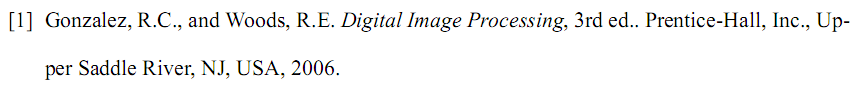
\includegraphics[width=\textwidth]{images/gonzalez.png}

این شیوه برای تعداد مراجع کم بد نیست اما اگر فرمت مراجع، ترتیب یا تعداد آنها را خواسته باشید تغییر دهید، به عنوان مثال ابتدا حرف اول نام نویسنده بیاید و سپس نام خانوادگی، باید همه کارها را به صورت دستی انجام دهید.
اگر مایلید کنترل کاملی بر مراجع خود داشته باشید و به راحتی بتوانید قالب مراجع خود را عوض کنید باید از \lr{Bib\TeX} استفاده کنید که درپیوست  \ref{App:RefMan} به  آن پرداخته خواهد شد.
!
را در فایل 
\lr{main.tex}،
غیرفعال%
\footnote{
برای غیرفعال کردن یک دستور، کافی است در ابتدای آن، یک علامت
\%
 بگذارید.
}
 کنید.  در غیر این صورت، ابتدا مطالب دو فصل اول  پردازش شده و سپس مطالب فصل ۳ پردازش می‌شود و این کار باعث طولانی شدن زمان اجرا می‌شود. هر زمان که خروجی کل \پ خود را خواستید تمام فصلها را از حالت توضیح خارج کنید.

\subsection{مراجع}
برای وارد کردن مراجع \پ خود، کافی است فایل 
\lr{MyReferences.bib}
را باز کرده و مراجع خود را مانند مراجع داخل آن، وارد کنید.  سپس از \lr{bibtex} برای تولید مراجع با قالب مناسب استفاده کنید. برای توضیحات بیشتر بخش \ref{Sec:Ref} و پیوست \ref{App:RefMan} را ببینید.
\subsection{مقاله‌های برگرفته از پارسا}
دانشجوهای مقطع ارشد و دکتری می‌توانند فهرست مقاله‌های برگرفته از پارسا را در فایل 
\lr{publications.bib}
وارد کنند و سپس آن‌ها را در فایل
\lr{papers.tex}
فراخوانی کنند.
\subsection{کارنامک}
كارنامک، نمایی كوتاه از كارهای علمـی و درجه‌های تحصـيلی دانش‌آموخته را نشـان می‌دهد و به زبان سوم شخص (غایب) نوشته‌ می‌شود. این بخش بـرای دانش‌آموختگان كارشناسی ارشد، اختياری و برای دانش‌آموختگان دكتری الزامی است. برای كسانی كـه پارسـا را به زبانی به‌جز فارسی می‌نویسند، این کارنامک نيز باید به همان زبان نوشته شود. برای مشاهده و ویرایش کارنامک فایل 
\lr{karnamak.tex}
را ببینید.
\subsection{واژه‌نامه فارسی به انگلیسی و برعکس}
برای وارد کردن واژه‌نامه فارسی به انگلیسی و برعکس، چنانچه کاربر مبتدی هستید، بهتر است مانند روش بکار رفته در فایل‌های 
\lr{dicfa2en}
و
\lr{dicen2fa}
عمل کنید. اما چنانچه کاربر پیشرفته هستید، بهتر است از بسته
\lr{glossaries}
استفاده کنید. راهنمای این بسته را می‌توانید به راحتی و با یک جستجوی ساده در اینترنت پیدا کنید.  به صورت پیش‌فرض از حالت پیشرفته برای ساخت واژه‌نامه‌ها استفاده شده است. به عنوان مثال اگر بخواهید کلمه‌هایی مانند "میانگین" و "واریانس" را به واژه‌نامه اضافه کنید از دستور
\verb!\inpdic{}{}!
استفاده کنید تا واژه‌های
\inpdic{میانگین}{Mean}
و 
\inpdic{واریانس}{Variance}
هم به پانوشت و هم به هر دو واژه‌نامه اضافه شوند. 

برای مشاهده خروجی این دو واژه‌نامه در ویرایشگر 
\lr{TeXstudio}
به منوی 
\[ \verb!Options > configure TeXstudio > Build! \]
مراجعه کنید و در پنجره سمت راست، بخش
\verb!User Commands!
با کلیک روی گزینه بعلاوه، یک دستور جدید با نام دلخواه مانند 
\verb!user0:glossary!
بسازید و به جای 
\verb!><unknown!
کد زیر را وارد و ذخیره کنید.
\begin{latin}
	\begin{verbatim}
		xindy -L persian-variant1 -C utf8 -I xindy -M %.xdy -t %.glg -o %.gls %.glo | 
		xindy -L persian-variant1 -C utf8 -I xindy -M %.xdy -t %.blg -o %.bls %.blo |
		xindy -L english -C utf8 -I xindy -M %.xdy -t %.alg -o %.acr %.acn>
	\end{verbatim}
\end{latin}
\noindent
حال برای اجرای دستور فوق از منوی 
\verb!User > Tools!
اقدام به اجرا کنید.
%\subsection{نمایه}
%برای وارد کردن نمایه، باید از 
%\lr{xindy}
%استفاده کنید. 
%%زیرا 
%%\lr{MakeIndex}
%%با حروف «گ»، «چ»، «پ»، «ژ» و «ک» مشکل دارد و ترتیب الفبایی این حروف را رعایت نمی‌کند. همچنین، فاصله بین هر گروه از کلمات در 
%%\lr{MakeIndex}،
%%به درستی رعایت نمی‌شود که باعث زشت شدن حروف‌چینی این قسمت می‌شود.
%در ویرایشگر 
%\lr{TeXstudio}
%می‌توان این کار را با استفاده از منوی 
%\verb!Index > Tools! 
%انجام داد. راهنمای چگونگی کار با 
%\lr{xindy} 
%را می‌توانید در ویدئوهای موجود در بسته آموزشی ببینید.

\section{اگر سوالی داشتم، از کی بپرسم؟}
 برای پرسیدن سوال‌های خود در مورد حروف‌چینی با زی‌پرشین،  می‌توانید به سایت‌های 
\hbox{\href{http://qa.parsilatex.com}{ پرسش و پاسخ پارسی‌لاتک}}%
\LTRfootnote{\url{http://qa.parsilatex.com}} 
و یا 
\hbox{\href{https://tex.stackexchange.com/questions}{\lr{Stack Exchange}}}%
\LTRfootnote{\url{https://tex.stackexchange.com/questions}}
مراجعه کنید. شما هم می‌توانید روزی به سوال‌های دیگران در این سایت جواب بدهید.

\section{جمع‌بندی}
در این فصل به بیان مقدمات نحوه استفاده از قالب پایان‌نامه/رساله دانشگاه رازی پرداخته شد. 
گرچه که مطالعه کامل این راهنما مقداری وقت شما را خواهد گرفت، اما مطمئن باشید از اتلاف وقت شما در ادامه کارتان تا حد زیادی جلوگیری خواهد کرد. 
در نوشتن متن حاضر سعی شده است بیشتر مواردی که عموماً دانشجوان با آن مواجه هستند ذکر شود. 
در ادامه نوشتار نمونه مواردی از درج تصویر، نمودار، کد برنامه، الگوریتم، توضیحات، منابع، فرمول، تعریف، قضیه، مثال و جدول آمده است. 
توصیه می‌شود یک کپی از کل فایل‌های این قالب را جداگانه از نسخه پایان‌نامه/رساله خود نگهداری نمایید تا در صورت نیاز بتوانید مراجعه فرمایید. 
همچنین توصیه اکید داریم که رفع خطاهایی که احتمالاً با آن مواجه می‌شوید را به آخر موکول نفرمایید و به محض برخورد با خطا، آن را اشکال‌زدایی نموده و 
خطا را برطرف فرمایید.

!
و
\verb!% !TeX root=main.tex
\chapter{آشنایی سریع با برخی دستورات لاتک}\label{Chap:latexIntro}
\thispagestyle{empty}
در این فصل ویژگی‌های مهم و پرکاربرد زی‌پرشین و لاتک معرفی می‌شود. برای راهنمایی بیشتر و به‌کاربردن ویژگی‌های پیشرفته‌تر به راهنمای زی‌پرشین و راهنمای لاتک مراجعه کنید. برای آگاهی از دستورات لاتک که این خروجی را تولید کرده‌اند فایل \lr{chapter2.tex} را ملاحظه فرمایید.
\footnote{بیشتر مطالب این بخش از مثال 
\lr{xepersian\_example.tex}
گرفته شده‌اند که توسط دوستمان آقای امیرمسعود پورموسی آماده شده بوده است.}

\section{بندها و زیرنویس‌ها}
هر جایی از نوشتهٔ خود، اگر می‌خواهید به سر سطر بروید و یک بند تازه را آغاز کنید، باید یک خط را خالی بگذارید
\footnote{یعنی دوبار باید کلید \lr{Enter} را بزنید.}
 مانند این:

حالا که یک بند تازه آغاز شده است، یک زیرنویس انگلیسی
\LTRfootnote{English Footnote!}
 هم می‌نویسیم!
\section{فرمول‌های ریاضی}\label{formula}

اینجا هم یک فرمول می‌آوریم که شماره دارد:
\begin{equation}\label{eq:yek}
A=\frac{c}{d}+\frac{q^2}{\sin(\omega t)+\Omega_{12}}
\end{equation}
در لاتک می‌توان به کمک فرمان 
\lr{\textbackslash label\{\}}
به هر فرمول یک نام نسبت داد. در فرمول بالا نام \lr{eq:yek} را برایش گذاشته‌ایم (پروندهٔ \lr{tex} همراه با این مثال را ببینید). این نام ما را قادر می‌کند که بعداً بتوانیم با فرمان
\lr{\textbackslash ref\{eq:yek\}}
به آن فرمول با شماره ارجاع دهیم. یعنی بنویسیم فرمول
 \eqref{eq:yek}. 
لاتک خودش شمارهٔ این فرمول‌ها را مدیریت می‌کند.\footnote{یعنی اگر بعداً فرمولی قبل از این فرمول بنویسیم، خودبه‌خود شمارهٔ این فرمول و شمارهٔ ارجاع‌ها به این فرمول یکی زیاد می‌شود. دیگر نگران شماره‌گذاری فرمول‌های خود نباشید!} این هم یک فرمول که شماره ندارد:
$$A=|\vec{a}\times \vec{b}| + \sum_{n=0}^\infty C_{ij}$$

این هم عبارتی ریاضی مانند 
$\sqrt{a^2+b^2}$
 که بین متن می‌آید.
\subsection{یک زیربخش}\label{zirbakhsh}

این زیربخش \ref{zirbakhsh} است؛ یعنی یک بخش درون بخش \ref{formula} است.
\subsubsection{یک زیرزیربخش}
این هم یک زیرزیربخش است. در لاتک می‌توانید بخش‌های تودرتو در نوشته‌تان تعریف کنید تا ساختار منطقی نوشته را به خوبی نشان دهید. می‌توانید به این بخش‌ها هم با شماره ارجاع دهید، مثلاً بخش فرمول‌های ریاضی شماره‌اش \ref{formula} است.
\section{نوشته‌های فارسی و انگلیسی مخلوط}
نوشتن یک کلمهٔ انگلیسی بین متن فارسی بدیهی است، مانند 
\lr{Example}
 در این جمله.
نوشتن یک عبارت چندکلمه‌ای مانند
 \lr{More than one word} کمی پیچیده‌تر است.

اگر ناگهان تصمیم بگیرید که یک بند کاملاً انگلیسی را بنویسید، باید:
\begin{latin}
This is an English paragraph from left to right. You can write as much as you want in it.
\end{latin}
\section{افزودن تصویر به نوشته}
پروندهٔ تصویر دلخواه خود را در کنار پروندهٔ \lr{tex} قرار دهید. سپس به روش زیر تصویر را در نوشتهٔ خود بیاورید:
\begin{latin}
\begin{verbatim}
\includegraphics{YourImageFileName}
\end{verbatim}
\end{latin}
به تصویرها هم مانند فرمول‌ها و بخش‌ها می‌توان با شماره ارجاع داد. مثلاً تصویر  \ref{fig:shir} یک شیر علاقه‌مند به لاتک را در حال دویدن نشان می‌دهد. برای جزئیات بیشتر دربارهٔ روش گذاشتن تصویرها در نوشته باید راهنماهای لاتک را بخوانید.
\begin{figure}%[ht]
\centerline{
\includegraphics[width=5cm]{images/lion}}
\caption{در این تصویر یک شیر علاقه‌مند به لاتک را در حال دویدن می‌بینید.}
\label{fig:shir}
\end{figure}

به تصویرها هم مانند فرمول‌ها و بخش‌ها می‌توان با شماره ارجاع داد. مثلاً تصویر بالا شماره‌اش \ref{fig:shir} است. برای جزئیات بیشتر دربارهٔ روش گذاشتن تصویرها در نوشته باید راهنماهای لاتک را بخوانید.

\section{محیط‌های شمارش و نکات}
برای فهرست‌کردن چندمورد، اگر ترتیب برایمان مهم نباشد:
\begin{itemize}
\item مورد یکم
\item مورد دوم
\item مورد سوم
\end{itemize}
و اگر ترتیب برایمان مهم باشد:
\begin{enumerate}
\item مورد یکم
\item مورد دوم
\item مورد سوم
\end{enumerate}
می‌توان موردهای تودرتو داشت:
\begin{enumerate}
\item مورد ۱
\item مورد ۲
\begin{enumerate}
\item مورد ۱ از ۲
\item مورد ۲ از ۲
\item مورد ۳ از ۲
\end{enumerate}
\item مورد ۳
\end{enumerate}
شماره‌گذاری این موردها را هم لاتک انجام می‌دهد.

\section{تعریف و قضیه}
برای ذکر تعریف، قضیه و مثال، مثالهای ذیل را ببینید.
\begin{definition}
مجموعه همه ارزیابی‌های  (پیوسته)  روی $(X,\tau)$، دامنه توانی احتمالی
\index{دامنه توانی احتمالی}
$ X $
نامیده می‌شود.
\end{definition}
\begin{theorem}[باناخ-آلااغلو]
\index{قضیه باناخ-آلااغلو}
اگر $ V $ یک همسایگی $ 0 $ در فضای برداری 
\index{فضای!برداری}
 توپولوژیکی $ X $ باشد و 
\begin{equation}\label{eq1}
K=\left\lbrace \Lambda \in X^{*}:|\Lambda x|\leqslant 1 ; \ \forall x\in V\right\rbrace,
\end{equation}
آنگاه $ K $،  ضعیف*-فشرده است که در آن، $ X^{*} $ دوگان
\index{فضای!دوگان}
 فضای برداری توپولوژیکی $ X $ است به ‌طوری که عناصر آن،  تابعی‌های 
خطی پیوسته
\index{تابعی خطی پیوسته}
 روی $X$ هستند.
\end{theorem}
\begin{proof}
	این یک اثبات است... در انتهای اثبات به صورت خودکار یک مربع خالی قرار می‌گیرد.
\end{proof}
\begin{corollary}
	این یک نتیجه است...
\end{corollary}
تساوی \eqref{eq1} یکی از مهم‌ترین تساوی‌ها در آنالیز تابعی است که در ادامه، به وفور از آن استفاده می‌شود.
\begin{example}
برای هر فضای مرتب، گردایه 
$$U:=\left\lbrace U\in O: U=\uparrow U\right\rbrace $$
از مجموعه‌های بالایی باز، یک توپولوژی تعریف می‌کند که از توپولوژی اصلی، درشت‌تر  است.
\end{example}
حال تساوی 
\begin{equation}\label{eq2}
\sum_{n=1}^{+\infty} 3^{n}x+7x=\int_{1}^{n}8nx+\exp{(2nx)}
\end{equation}
را در نظر بگیرید. با مقایسه تساوی \eqref{eq2} با تساوی \eqref{eq1} می‌توان نتیجه گرفت که ...


\section{چگونگی نوشتن و ارجاع به مراجع}\label{Sec:Ref}

در لاتک به راحتی می‌توان مراجع خود را نوشت و به آنها ارجاع داد. به عنوان مثال برای معرفی یک کتاب مانند کتاب گنزالس \citep{Gonzalez02book} به عنوان یک مرجع می‌توان آنرا به صورت زیر معرفی نمود:

\singlespacing
\begin{LTR}
\begin{verbatim}
\bibitem{Gonzalez02book}
Gonzalez, R.C., and Woods, R.E. {\em Digital Image Processing}, 3rd ed..
Prentice-Hall, Inc., Upper Saddle River, NJ, USA, 2006.
\end{verbatim}
\end{LTR}
\doublespacing

در دستورات فوق \lr{Gonzalez02book}  برچسبی است که به این مرجع داده شده است و با استفاده از دستور 
\verb!\cite{Gonzalez02book}!
می‌توان به آن ارجاع داد؛ بدون این که شماره‌اش را در فهرست مراجع‌مان بدانیم.

اگر این اولین مرجع ما باشد در قسمت مراجع به صورت زیر خواهد آمد:\\
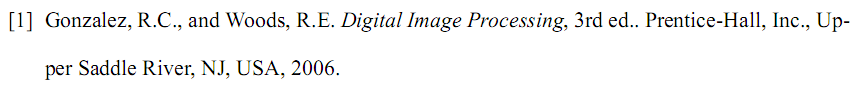
\includegraphics[width=\textwidth]{images/gonzalez.png}

این شیوه برای تعداد مراجع کم بد نیست اما اگر فرمت مراجع، ترتیب یا تعداد آنها را خواسته باشید تغییر دهید، به عنوان مثال ابتدا حرف اول نام نویسنده بیاید و سپس نام خانوادگی، باید همه کارها را به صورت دستی انجام دهید.
اگر مایلید کنترل کاملی بر مراجع خود داشته باشید و به راحتی بتوانید قالب مراجع خود را عوض کنید باید از \lr{Bib\TeX} استفاده کنید که درپیوست  \ref{App:RefMan} به  آن پرداخته خواهد شد.
!
را در فایل 
\lr{main.tex}،
غیرفعال%
\footnote{
برای غیرفعال کردن یک دستور، کافی است در ابتدای آن، یک علامت
\%
 بگذارید.
}
 کنید.  در غیر این صورت، ابتدا مطالب دو فصل اول  پردازش شده و سپس مطالب فصل ۳ پردازش می‌شود و این کار باعث طولانی شدن زمان اجرا می‌شود. هر زمان که خروجی کل \پ خود را خواستید تمام فصلها را از حالت توضیح خارج کنید.

\subsection{مراجع}
برای وارد کردن مراجع \پ خود، کافی است فایل 
\lr{MyReferences.bib}
را باز کرده و مراجع خود را مانند مراجع داخل آن، وارد کنید.  سپس از \lr{bibtex} برای تولید مراجع با قالب مناسب استفاده کنید. برای توضیحات بیشتر بخش \ref{Sec:Ref} و پیوست \ref{App:RefMan} را ببینید.
\subsection{مقاله‌های برگرفته از پارسا}
دانشجوهای مقطع ارشد و دکتری می‌توانند فهرست مقاله‌های برگرفته از پارسا را در فایل 
\lr{publications.bib}
وارد کنند و سپس آن‌ها را در فایل
\lr{papers.tex}
فراخوانی کنند.
\subsection{کارنامک}
كارنامک، نمایی كوتاه از كارهای علمـی و درجه‌های تحصـيلی دانش‌آموخته را نشـان می‌دهد و به زبان سوم شخص (غایب) نوشته‌ می‌شود. این بخش بـرای دانش‌آموختگان كارشناسی ارشد، اختياری و برای دانش‌آموختگان دكتری الزامی است. برای كسانی كـه پارسـا را به زبانی به‌جز فارسی می‌نویسند، این کارنامک نيز باید به همان زبان نوشته شود. برای مشاهده و ویرایش کارنامک فایل 
\lr{karnamak.tex}
را ببینید.
\subsection{واژه‌نامه فارسی به انگلیسی و برعکس}
برای وارد کردن واژه‌نامه فارسی به انگلیسی و برعکس، چنانچه کاربر مبتدی هستید، بهتر است مانند روش بکار رفته در فایل‌های 
\lr{dicfa2en}
و
\lr{dicen2fa}
عمل کنید. اما چنانچه کاربر پیشرفته هستید، بهتر است از بسته
\lr{glossaries}
استفاده کنید. راهنمای این بسته را می‌توانید به راحتی و با یک جستجوی ساده در اینترنت پیدا کنید.  به صورت پیش‌فرض از حالت پیشرفته برای ساخت واژه‌نامه‌ها استفاده شده است. به عنوان مثال اگر بخواهید کلمه‌هایی مانند "میانگین" و "واریانس" را به واژه‌نامه اضافه کنید از دستور
\verb!\inpdic{}{}!
استفاده کنید تا واژه‌های
\inpdic{میانگین}{Mean}
و 
\inpdic{واریانس}{Variance}
هم به پانوشت و هم به هر دو واژه‌نامه اضافه شوند. 

برای مشاهده خروجی این دو واژه‌نامه در ویرایشگر 
\lr{TeXstudio}
به منوی 
\[ \verb!Options > configure TeXstudio > Build! \]
مراجعه کنید و در پنجره سمت راست، بخش
\verb!User Commands!
با کلیک روی گزینه بعلاوه، یک دستور جدید با نام دلخواه مانند 
\verb!user0:glossary!
بسازید و به جای 
\verb!><unknown!
کد زیر را وارد و ذخیره کنید.
\begin{latin}
	\begin{verbatim}
		xindy -L persian-variant1 -C utf8 -I xindy -M %.xdy -t %.glg -o %.gls %.glo | 
		xindy -L persian-variant1 -C utf8 -I xindy -M %.xdy -t %.blg -o %.bls %.blo |
		xindy -L english -C utf8 -I xindy -M %.xdy -t %.alg -o %.acr %.acn>
	\end{verbatim}
\end{latin}
\noindent
حال برای اجرای دستور فوق از منوی 
\verb!User > Tools!
اقدام به اجرا کنید.
%\subsection{نمایه}
%برای وارد کردن نمایه، باید از 
%\lr{xindy}
%استفاده کنید. 
%%زیرا 
%%\lr{MakeIndex}
%%با حروف «گ»، «چ»، «پ»، «ژ» و «ک» مشکل دارد و ترتیب الفبایی این حروف را رعایت نمی‌کند. همچنین، فاصله بین هر گروه از کلمات در 
%%\lr{MakeIndex}،
%%به درستی رعایت نمی‌شود که باعث زشت شدن حروف‌چینی این قسمت می‌شود.
%در ویرایشگر 
%\lr{TeXstudio}
%می‌توان این کار را با استفاده از منوی 
%\verb!Index > Tools! 
%انجام داد. راهنمای چگونگی کار با 
%\lr{xindy} 
%را می‌توانید در ویدئوهای موجود در بسته آموزشی ببینید.

\section{اگر سوالی داشتم، از کی بپرسم؟}
 برای پرسیدن سوال‌های خود در مورد حروف‌چینی با زی‌پرشین،  می‌توانید به سایت‌های 
\hbox{\href{http://qa.parsilatex.com}{ پرسش و پاسخ پارسی‌لاتک}}%
\LTRfootnote{\url{http://qa.parsilatex.com}} 
و یا 
\hbox{\href{https://tex.stackexchange.com/questions}{\lr{Stack Exchange}}}%
\LTRfootnote{\url{https://tex.stackexchange.com/questions}}
مراجعه کنید. شما هم می‌توانید روزی به سوال‌های دیگران در این سایت جواب بدهید.

\section{جمع‌بندی}
در این فصل به بیان مقدمات نحوه استفاده از قالب پایان‌نامه/رساله دانشگاه رازی پرداخته شد. 
گرچه که مطالعه کامل این راهنما مقداری وقت شما را خواهد گرفت، اما مطمئن باشید از اتلاف وقت شما در ادامه کارتان تا حد زیادی جلوگیری خواهد کرد. 
در نوشتن متن حاضر سعی شده است بیشتر مواردی که عموماً دانشجوان با آن مواجه هستند ذکر شود. 
در ادامه نوشتار نمونه مواردی از درج تصویر، نمودار، کد برنامه، الگوریتم، توضیحات، منابع، فرمول، تعریف، قضیه، مثال و جدول آمده است. 
توصیه می‌شود یک کپی از کل فایل‌های این قالب را جداگانه از نسخه پایان‌نامه/رساله خود نگهداری نمایید تا در صورت نیاز بتوانید مراجعه فرمایید. 
همچنین توصیه اکید داریم که رفع خطاهایی که احتمالاً با آن مواجه می‌شوید را به آخر موکول نفرمایید و به محض برخورد با خطا، آن را اشکال‌زدایی نموده و 
خطا را برطرف فرمایید.

			% فصل اول: مقدمه
% !TeX root=main.tex
\chapter{آشنایی سریع با برخی دستورات لاتک}\label{Chap:latexIntro}
\thispagestyle{empty}
در این فصل ویژگی‌های مهم و پرکاربرد زی‌پرشین و لاتک معرفی می‌شود. برای راهنمایی بیشتر و به‌کاربردن ویژگی‌های پیشرفته‌تر به راهنمای زی‌پرشین و راهنمای لاتک مراجعه کنید. برای آگاهی از دستورات لاتک که این خروجی را تولید کرده‌اند فایل \lr{chapter2.tex} را ملاحظه فرمایید.
\footnote{بیشتر مطالب این بخش از مثال 
\lr{xepersian\_example.tex}
گرفته شده‌اند که توسط دوستمان آقای امیرمسعود پورموسی آماده شده بوده است.}

\section{بندها و زیرنویس‌ها}
هر جایی از نوشتهٔ خود، اگر می‌خواهید به سر سطر بروید و یک بند تازه را آغاز کنید، باید یک خط را خالی بگذارید
\footnote{یعنی دوبار باید کلید \lr{Enter} را بزنید.}
 مانند این:

حالا که یک بند تازه آغاز شده است، یک زیرنویس انگلیسی
\LTRfootnote{English Footnote!}
 هم می‌نویسیم!
\section{فرمول‌های ریاضی}\label{formula}

اینجا هم یک فرمول می‌آوریم که شماره دارد:
\begin{equation}\label{eq:yek}
A=\frac{c}{d}+\frac{q^2}{\sin(\omega t)+\Omega_{12}}
\end{equation}
در لاتک می‌توان به کمک فرمان 
\lr{\textbackslash label\{\}}
به هر فرمول یک نام نسبت داد. در فرمول بالا نام \lr{eq:yek} را برایش گذاشته‌ایم (پروندهٔ \lr{tex} همراه با این مثال را ببینید). این نام ما را قادر می‌کند که بعداً بتوانیم با فرمان
\lr{\textbackslash ref\{eq:yek\}}
به آن فرمول با شماره ارجاع دهیم. یعنی بنویسیم فرمول
 \eqref{eq:yek}. 
لاتک خودش شمارهٔ این فرمول‌ها را مدیریت می‌کند.\footnote{یعنی اگر بعداً فرمولی قبل از این فرمول بنویسیم، خودبه‌خود شمارهٔ این فرمول و شمارهٔ ارجاع‌ها به این فرمول یکی زیاد می‌شود. دیگر نگران شماره‌گذاری فرمول‌های خود نباشید!} این هم یک فرمول که شماره ندارد:
$$A=|\vec{a}\times \vec{b}| + \sum_{n=0}^\infty C_{ij}$$

این هم عبارتی ریاضی مانند 
$\sqrt{a^2+b^2}$
 که بین متن می‌آید.
\subsection{یک زیربخش}\label{zirbakhsh}

این زیربخش \ref{zirbakhsh} است؛ یعنی یک بخش درون بخش \ref{formula} است.
\subsubsection{یک زیرزیربخش}
این هم یک زیرزیربخش است. در لاتک می‌توانید بخش‌های تودرتو در نوشته‌تان تعریف کنید تا ساختار منطقی نوشته را به خوبی نشان دهید. می‌توانید به این بخش‌ها هم با شماره ارجاع دهید، مثلاً بخش فرمول‌های ریاضی شماره‌اش \ref{formula} است.
\section{نوشته‌های فارسی و انگلیسی مخلوط}
نوشتن یک کلمهٔ انگلیسی بین متن فارسی بدیهی است، مانند 
\lr{Example}
 در این جمله.
نوشتن یک عبارت چندکلمه‌ای مانند
 \lr{More than one word} کمی پیچیده‌تر است.

اگر ناگهان تصمیم بگیرید که یک بند کاملاً انگلیسی را بنویسید، باید:
\begin{latin}
This is an English paragraph from left to right. You can write as much as you want in it.
\end{latin}
\section{افزودن تصویر به نوشته}
پروندهٔ تصویر دلخواه خود را در کنار پروندهٔ \lr{tex} قرار دهید. سپس به روش زیر تصویر را در نوشتهٔ خود بیاورید:
\begin{latin}
\begin{verbatim}
\includegraphics{YourImageFileName}
\end{verbatim}
\end{latin}
به تصویرها هم مانند فرمول‌ها و بخش‌ها می‌توان با شماره ارجاع داد. مثلاً تصویر  \ref{fig:shir} یک شیر علاقه‌مند به لاتک را در حال دویدن نشان می‌دهد. برای جزئیات بیشتر دربارهٔ روش گذاشتن تصویرها در نوشته باید راهنماهای لاتک را بخوانید.
\begin{figure}%[ht]
\centerline{
\includegraphics[width=5cm]{images/lion}}
\caption{در این تصویر یک شیر علاقه‌مند به لاتک را در حال دویدن می‌بینید.}
\label{fig:shir}
\end{figure}

به تصویرها هم مانند فرمول‌ها و بخش‌ها می‌توان با شماره ارجاع داد. مثلاً تصویر بالا شماره‌اش \ref{fig:shir} است. برای جزئیات بیشتر دربارهٔ روش گذاشتن تصویرها در نوشته باید راهنماهای لاتک را بخوانید.

\section{محیط‌های شمارش و نکات}
برای فهرست‌کردن چندمورد، اگر ترتیب برایمان مهم نباشد:
\begin{itemize}
\item مورد یکم
\item مورد دوم
\item مورد سوم
\end{itemize}
و اگر ترتیب برایمان مهم باشد:
\begin{enumerate}
\item مورد یکم
\item مورد دوم
\item مورد سوم
\end{enumerate}
می‌توان موردهای تودرتو داشت:
\begin{enumerate}
\item مورد ۱
\item مورد ۲
\begin{enumerate}
\item مورد ۱ از ۲
\item مورد ۲ از ۲
\item مورد ۳ از ۲
\end{enumerate}
\item مورد ۳
\end{enumerate}
شماره‌گذاری این موردها را هم لاتک انجام می‌دهد.

\section{تعریف و قضیه}
برای ذکر تعریف، قضیه و مثال، مثالهای ذیل را ببینید.
\begin{definition}
مجموعه همه ارزیابی‌های  (پیوسته)  روی $(X,\tau)$، دامنه توانی احتمالی
\index{دامنه توانی احتمالی}
$ X $
نامیده می‌شود.
\end{definition}
\begin{theorem}[باناخ-آلااغلو]
\index{قضیه باناخ-آلااغلو}
اگر $ V $ یک همسایگی $ 0 $ در فضای برداری 
\index{فضای!برداری}
 توپولوژیکی $ X $ باشد و 
\begin{equation}\label{eq1}
K=\left\lbrace \Lambda \in X^{*}:|\Lambda x|\leqslant 1 ; \ \forall x\in V\right\rbrace,
\end{equation}
آنگاه $ K $،  ضعیف*-فشرده است که در آن، $ X^{*} $ دوگان
\index{فضای!دوگان}
 فضای برداری توپولوژیکی $ X $ است به ‌طوری که عناصر آن،  تابعی‌های 
خطی پیوسته
\index{تابعی خطی پیوسته}
 روی $X$ هستند.
\end{theorem}
\begin{proof}
	این یک اثبات است... در انتهای اثبات به صورت خودکار یک مربع خالی قرار می‌گیرد.
\end{proof}
\begin{corollary}
	این یک نتیجه است...
\end{corollary}
تساوی \eqref{eq1} یکی از مهم‌ترین تساوی‌ها در آنالیز تابعی است که در ادامه، به وفور از آن استفاده می‌شود.
\begin{example}
برای هر فضای مرتب، گردایه 
$$U:=\left\lbrace U\in O: U=\uparrow U\right\rbrace $$
از مجموعه‌های بالایی باز، یک توپولوژی تعریف می‌کند که از توپولوژی اصلی، درشت‌تر  است.
\end{example}
حال تساوی 
\begin{equation}\label{eq2}
\sum_{n=1}^{+\infty} 3^{n}x+7x=\int_{1}^{n}8nx+\exp{(2nx)}
\end{equation}
را در نظر بگیرید. با مقایسه تساوی \eqref{eq2} با تساوی \eqref{eq1} می‌توان نتیجه گرفت که ...


\section{چگونگی نوشتن و ارجاع به مراجع}\label{Sec:Ref}

در لاتک به راحتی می‌توان مراجع خود را نوشت و به آنها ارجاع داد. به عنوان مثال برای معرفی یک کتاب مانند کتاب گنزالس \citep{Gonzalez02book} به عنوان یک مرجع می‌توان آنرا به صورت زیر معرفی نمود:

\singlespacing
\begin{LTR}
\begin{verbatim}
\bibitem{Gonzalez02book}
Gonzalez, R.C., and Woods, R.E. {\em Digital Image Processing}, 3rd ed..
Prentice-Hall, Inc., Upper Saddle River, NJ, USA, 2006.
\end{verbatim}
\end{LTR}
\doublespacing

در دستورات فوق \lr{Gonzalez02book}  برچسبی است که به این مرجع داده شده است و با استفاده از دستور 
\verb!\cite{Gonzalez02book}!
می‌توان به آن ارجاع داد؛ بدون این که شماره‌اش را در فهرست مراجع‌مان بدانیم.

اگر این اولین مرجع ما باشد در قسمت مراجع به صورت زیر خواهد آمد:\\
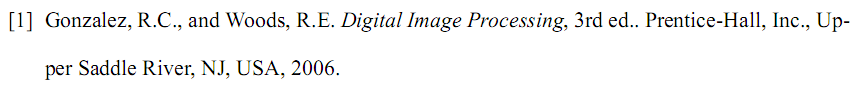
\includegraphics[width=\textwidth]{images/gonzalez.png}

این شیوه برای تعداد مراجع کم بد نیست اما اگر فرمت مراجع، ترتیب یا تعداد آنها را خواسته باشید تغییر دهید، به عنوان مثال ابتدا حرف اول نام نویسنده بیاید و سپس نام خانوادگی، باید همه کارها را به صورت دستی انجام دهید.
اگر مایلید کنترل کاملی بر مراجع خود داشته باشید و به راحتی بتوانید قالب مراجع خود را عوض کنید باید از \lr{Bib\TeX} استفاده کنید که درپیوست  \ref{App:RefMan} به  آن پرداخته خواهد شد.
		% فصل دوم: آشنایی مقدماتی با لاتک
% فصل سوم
% !TeX root=main.tex
\chapter{مشخصه و دستورالعمل نگارش یک گزارش علمی}\label{Chap:thesis}
\thispagestyle{empty}
این یک توضیح کوتاه است...
\section{مشخصه یک گزارش علمی}
اگرچه برای همه انواع نوشته‌ها، مشخصات و ویژگی‌های واحد و معینی نمی‌توان ذكر كرد، با این حال در یک پایان نامه یا گزارش علمی باید نکات و موارد کلی که در این فصل ذکر می‌شود، بطور کامل رعایت شده باشد. 
دقت كنید كه پس از عنوان فصل باید حداقل توضیحی کوتاه در مورد موضوع نوشته شود و نمی‌توان مستقیماً بعد از آن عنوان بخش را نوشت و همین طور پس از عناوین بخش‌ها و زیربخش‌ها.(مانند دستورالعمل حاضر)
\subsection{برخورداری از غنای علمی }
یك پایان نامه باید پیش از هر چیز به‌لحاظ علمی از غنای لازم برخوردار باشد. یعنی هدف و پیام روشنی داشته باشد و از پیش‌زمینه علمی، بیان دلایل علمی، ارجاعات مورد نیاز و نتیجه‌گیری شفاف بهره ببرد. 
\subsection{ارجاع به‌موقع و صحیح به منابع دیگر}
هر جمله‌ای که در یک پایان نامه نوشته می‌شود یا یک جمله کاملاً بدیهی است یا باید دلیل آن بیان شود و یا اینکه باید به منبعی که آن موضوع را نقل یا اثبات کرده، ارجاع داده شود. اگر مطلب یا گفتاری از منبعی عیناً در گزارش نقل می‌شود، باید آن مطلب داخل گیومه قرار گیرد و با ذكر ماخذ و شماره صفحه، به آن اشاره گردد.
\subsection{ساده‌نویسی}
سادگی از ضروریات یك نوشته است. نویسنده باید ساده، روان و در عین حال شیوا و رسا بنویسد و عبارات مبهم، جملات پیچیده و كلمات نامأنوس در نوشته خود به‌كار نبرد. اگر چه افراط در این امر نیز، به شیوایی نوشته صدمه می‌زند. به‌كارگیری لغات و اصطلاحات دشوار و دور از ذهن و عبارات و جملات نامنظم و مبهم موجب ایجاد اشكال در فهم خواننده خواهد شد‌. 

برای ساده‌نویسی باید در حد امكان از به‌كارگیری كلمات «می‌بایست»، «بایستی»، «گردید»، «بوده باشد» و مانند آنها كه تكلف‌آور، غلط مصطلح و یا غیرشیوا هستند، به‌جای «باید»، «است»، «شد» و مثل آنها، اجتناب شود‌.‌ همین‌طور، «در‌جهت» نمی‌تواند جایگزین خوبی برای كلمه روانی مثل «برای» باشد‌. ‌كلمات و جملات روان و ساده می‌توانند اغلب مفاهیم را براحتی منتقل كنند‌.‌     
 
      دقت در تنظیم بندها (پاراگراف‌ها) نیز كمك شایانی به روانی و سادگی فهم مطلب می‌كند‌.‌ بندهای طولانی نیز مانند جملات طولانی می‌توانند خسته‌كننده باشند و خواننده را سردرگم كنند‌.‌ یك بند نباید کمتر از سه یا چهار سطر یا بیشتر از 10 تا 15 سطر باشد.‌ 
      
\subsubsection{وحدت موضوع}
نویسنده باید در سراسر نوشته از اصل موضوع دور نیافتد و تمام بحث‌ها، مثال‌ها و اجزای نوشته با هماهنگی كامل، پیرامون موضوع اصلی باشد و تاثیری واحد در ذهن خواننده القا كند. 
\subsubsection{ اختصار}
پایان نامه یا گزارش علمی باید در حد امكان، مختصر و مفید باشد و از بحث‌های غیر ضروری در آن پرهیز شود. نوشتن مطالب ارزشمندی كه هیچ ربطی به موضوع ندارد، فاقد ارزش علمی است.
\subsubsection{رعایت نكات دستوری و نشانه‌گذاری}
در سراسر پایان نامه باید قواعد دستوری رعایت شود و اركان و اجزای جمله در جای مناسب خود آورده شود. همچنین رعایت قواعد نشانه‌گذاری سبب می‌شود كه بیان نویسنده روشن باشد و خواننده به سهولت و با کمترین صرف انرژی مطالب را مطالعه و درک كند.
\subsubsection{توجه به معلومات ذهنی مخاطب}
نویسنده باید همواره مخاطب خود را در برابر خود تصور كند و با توجه به معلومات ذهنی مخاطب  تمامی پیش‌نیازهای لازم برای درک مطالب مورد بحث را، از پیش برای مخاطب فراهم كند.
\subsubsection{رعایت مراحل اصولی نگارش}
هر کار علمی زمانی به بهترین شکل قابل انجام است که بر اساس یک برنامه‌ریزی مشخص انجام شود. تهیه یک متن علمی با کیفیت نیز نیازمند برنامه‌ریزی مناسب و اجرای منظم آن می‌باشد. مراحل نگارش را عموماً می‌توان به ترتیب زیر درنظر گرفت:
\begin{itemize}
\item 
	تهیه فهرستی از عناوین اصلی و فرعی که باید نوشته شود
\item 
اولویت‌بندی و تعیین ترتیب منطقی فصل‌ها و بخش‌های گزارش
\item
گردآوری اطلاعات اولیه راجع به هر بخش و زیربخش
\item
تدوین مطالب جدیدی که باید به قلم نگارنده به گزارش اضافه شود
\item
ماشین‌(تایپ)كردن مطالب با رعایت کامل نکاتی که در این دستورالعمل آموزش داده می‌شود
\end{itemize}	
رعایت نظم و ترتیب در اجرای مراحل سیستماتیک فوق هم فرآیند تهیه پایان نامه یا گزارش علمی را برای نگارنده آسان می‌کند و هم کیفیت نگارش را به میزان قابل توجهی افزایش می‌دهد.
\section{نگارش صحیح}
نگارش صحیح یک پایان نامه در فهم آسان آن بسیار موثر است. در این بخش مهمترین قواعد نگارشی که باید مورد توجه جدی نگارنده قرار گیرد، به اختصار بیان می‌شود. این قواعد را می‌توان در محورهای اصلی زیر دسته‌بندی کرد: 
\begin{itemize}
	\item 
	فارسی‌نویسی
	\item
	رعایت املای صحیح
	\item
	رعایت قواعد نشانه‌گذاری
\end{itemize}
\subsection{فارسی‌نویسی}
در حد امكان سعی كنید به جای كلمات غیر‌فارسی از معادل فارسی آنها استفاده كنید، به‌ویژه در مواردی كه معادل فارسی مصطلح و رایج است‌.‌ به‌طور مثال استفاده از كلمه «لذا» به‌جای «برای همین» یا «به‌همین دلیل» توجیهی ندارد‌. همچنین كلمه «پردازش» زیباتر از «پروسس» و معادل فارسی «ریز‌پردازنده» مناسب‌تر از «میكروپروسسور» است‌.‌ در این‌گونه موارد چنانچه احتمال عدم آشنایی خواننده با معادل فارسی وجود دارد، یا اصطلاح غیر‌فارسی معمول‌تر است، در اولین ظهور كلمه فارسی، اصل غیر‌فارسی آن به‌صورت پاورقی آورده شود‌.‌ اگر به‌ناچار باید كلمات انگلیسی در لابه‌لای جملات گنجانده شوند، از هر طرف یك فاصله بین آنها و كلمات فارسی پیش و پس از آنها در‌نظر گرفته شود‌.‌ چنانچه در پایان نامه از مختصر‌نویسی  
\LTRfootnote{Abbreviation}
استفاده شود، لازم است در اولین استفاده، تفصیل آن در پاورقی آورده شود‌.‌ 
مثلاً: همگی می‌دانیم که از سیستم تعیین موقعیت فراگیر 
(\lr{GPS}\LTRfootnote{Global Positioning System})
می‌توان برای تعیین موقعیت جغرافیایی یک وسیله پرنده استفاده کرد.
\subsection{رعایت املای صحیح فارسی}
رعایت املای صحیح فارسی به مطالعه و درك راحت‌تر كمك می‌كند. همچنین در نوشته‌های فارسی باید در حد امكان از همزه « ء، أ، ؤ، ة، إ، ئ» استفاده نشود‌.‌ به‌عنوان مثال «اجزاء هواپیما» و «آئین نگارش» ناصحیح، اما «اجزای هواپیما» و «آیین نگارش» صحیح هستند.‌
\subsection{رعایت قواعد نشانه‌گذاری}
منظور از نشانه‌گذاری به‌كار‌بردن علامت‌ها و نشانه‌هایی است كه خواندن و فهم درست یک جمله را ممکن و آسان می‌كند. در ادامه نشانه‌های معمول و متداول در زبان فارسی و موارد کاربرد آنها به اختصار معرفی می‌شوند.
\subsubsection{ویرگول}
ویرگول نشانه ضرورت یک مكث كوتاه است و در موارد زیر به‌كار می‌رود:
\begin{itemize}
	\item 
	در میان دو كلمه كه احتمال داده شود خواننده آنها را با كسره اضافه بخواند، یا نبودن ویرگول موجب بروز اشتباه در خواندن جمله شود.
	\item
	در موردی كه كلمه یا عبارتی به‌‌‌‌عنوان توضیح، در ضمن یک جمله آورده شود. مثلاً برای کنترل وضعیت فضاپیماها، به‌دلیل آن‌که در خارج از جو هستند، نمی‌توان از بالک‌های آیرودینامیکی استفاده کرد.
	\item
	جدا‌كردن بخش‌های مختلف یك نشانی یا یک مرجع
	\item
موارد دیگر از این قبیل
	پیش از ویرگول نباید فاصله گذاشته شود و پس از آن یك فاصله لازم است و بیشتر از آن صحیح نیست.
\end{itemize}
\subsubsection{نقطه}
نقطه نشانه پایان یک جمله است. پیش از نقطه نباید فاصله گذاشته شود و پس از آن یك فاصله لازم است و بیشتر از آن صحیح نیست. 
\subsubsection{دو نقطه}
موارد كاربرد دونقطه عبارتند از:
\begin{itemize}
	\item 
	پیش از نقل قول مستقیم
	\item 
	پیش از بیان تفصیل مطلبی كه به اجمال به آن اشاره شده ‌است.
	\item 
	پس از واژه‌ای كه معنی آن در برابرش آورده و نوشته می‌شود.
	\item 
	پس از كلمات تفسیر‌كننده از قبیل «یعنی» و ...
\end{itemize}	
پیش از دونقطه نباید فاصله گذاشته شود و پس از آن یك فاصله لازم است و بیشتر از آن صحیح نیست.
\subsubsection{گیومه}
موارد كاربرد گیومه عبارتند از:
\begin{itemize}
	\item 
وقتی كه عین گفته یا نوشته كسی را در ضمن نوشته و مطلب خود می‌آوریم. 
	و در آغاز و پایان كلمات و اصطلاحات علمی و یا هر كلمه و عبارتی كه باید به‌صورت ممتاز از قسمت‌های دیگر نشان داده شود.
	\item
	در ذكر عنوان مقاله‌ها، رساله‌ها، اشعار، روزنامه‌ها و ...
\end{itemize}
\subsubsection{نشانه پرسشی}
پیش از «؟» نباید فاصله گذاشته شود و پس از آن یك فاصله لازم است و بیشتر از آن صحیح نیست. 
\subsubsection{خط تیره}
موارد كاربرد خط تیره عبارتند از:
\begin{itemize}
	\item 
جدا‌كردن عبارت‌های توضیحی، بدل، عطف بیان و ...
	\item 
به‌جای حرف اضافه «تا» و «به» بین تاریخ‌ها، اعداد و كلمات
\end{itemize}
\subsubsection{پرانتز }
موارد كاربرد پرانتز عبارتند از:
\begin{itemize}
\item 
به‌معنی «یا» و «یعنی» و وقتی كه یک كلمه یا عبارت را برای توضیح بیشتر كلام بیاورند.	
\item
وقتی كه نویسنده بخواهد آگاهی‌های بیشتر (اطلاعات تكمیلی) به خواننده عرضه كند.		
\item
		برای ذكر مرجع در پایان مثال‌ها و شواهد.	
\end{itemize}	
\begin{example}
	بین کلمه یا عبارت داخل پرانتز و پرانتز باز و بسته نباید فاصله وجود داشته باشد.
\end{example}

\subsubsection{جدانوشتن كلمات بدون گذاشتن فاصله بین آنها}
گاهی لازم است اجزای یك كلمه از یكدیگر جدا نوشته شوند، بدون آنكه بین آنها فاصله گذاشته شود (مثل كلمه «می‌شود» یا «جدانوشتن»). به این منظور بین دو بخش كلمه مورد نظر از نیم‌فاصله
(\lr{SS})
 استفاده شود. برای ایجاد نیم‌فاصله توسط ویرایشگر 
\lr{TeXstudio}،
ابتدا به منوی 
\begin{latin}
\verb!Macros > Edit Macros...!	
\end{latin}
مراجعه و مانند شکل
\ref{fig:half}
عمل می‌کنیم. در نتیجه با توجه به مرحله چهارم شکل با فشردن کلیدهای
\verb!Ctrl+Shift+2!
می‌توان نیم‌فاصله تولید کرد.
\begin{figure}%[ht]
	\centerline{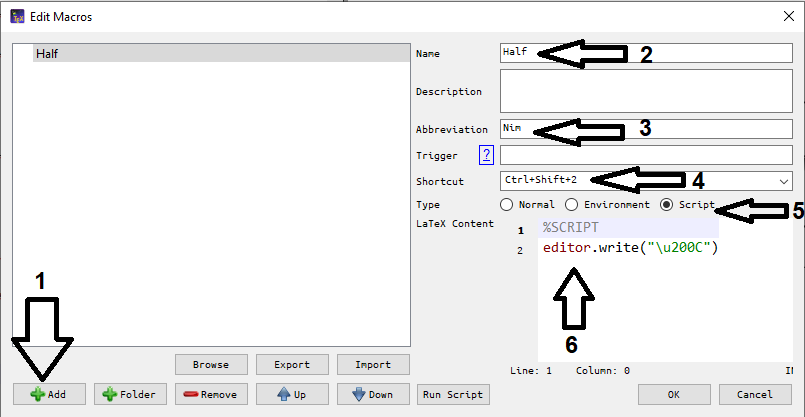
\includegraphics[width=15cm]{images/half}}
	\caption{در این تصویر یک شیر علاقه‌مند به لاتک را در حال دویدن می‌بینید.}
	\label{fig:half}
\end{figure}
 
تقریباً تمامی كلمات مركب در زبان فارسی باید از هم جدا نوشته شوند؛ به استثنای صفات فاعلی مانند «عملگر»، «باغبان» و یا «دانشمند» و كلماتی نظیر «اینكه»، «آنها». در ادامه به نمونه‌هایی از مواردی كه باید اجزای یك كلمه جدا، اما بدون فاصله نوشته شوند، اشاره می‌شود‌.

1-	در افعال مضارع و ماضی استمراری كه با «می» شروع می‌شوند، لازم است كه در عین جدا نوشتن، «می» از بخش بعدی فعل جدا نیافتد‌.‌ برای این منظور باید از «فاصله متصل» استفاده و «می» در اول فعل با SS از آن جدا شود.‌ به‌طور مثال «می‌شود» به‌جای «می شود». 

2-	«ها»ی جمع باید از كلمه جمع بسته‌شده جدا نوشته شود؛ مگر در برخی كلمات مانند «آنها». این امر در مورد كلمات غیر‌فارسی كه وارد زبان فارسی شده‌اند و با حرف «ها» جمع بسته می‌شوند، مانند «كانال‌ها» یا «فرمول‌ها» مورد تاكید است.

3-	حروف اضافه مانند «به» وقتی به‌صورت تركیب ثابت همراه كلمه پس از خود آورده می‌شوند، بهتر است با SS از آن جدا شوند‌.‌ مانند «به‌صورت»، «به‌عنوان» و «به‌‌‌لحاظ»‌.‌ لازم به ذكر است هنگامی كه حرف اضافه «به» با كلمه پس از خود معنای قیدی داشته باشد، مثل «بشدت» یا «بسادگی»، بهتر است كه به‌صورت چسبیده نوشته شود‌.

4-	كلمات فارسی نباید با قواعد عربی جمع بسته شوند؛ پس «پیشنهادها» صحیح و «پیشنهادات» اشتباه است‌.‌

5-	اسم‌ها و صفت‌های دو‌قسمتی مثل «خط‌چین» و «نوشته‌شده» با SS از هم جدا می‌شود‌.‌

6-	شناسه‌ها با SS از كلمه اصلی جدا می‌شود‌.‌ مثل «شده‌اند»‌ و «شده‌است». 

7-	‌ «است» هنگامی كه نقش شناسه را داشته باشد توسط SS از قسمت اصلی جدا می‌شود‌.‌ مانند «گفته‌است»‌.

8-	بند پیشین نباید باعث افراط در استفاده از فاصله متصل شود. مثلاً عبارت «نوشته می‌شود‌« صحیح و عبارت «نوشته‌می‌شود» ناصحیح است. 

9-	فعل‌های دو‌كلمه‌ای كه معنای اجزای آنها كاملاً با معنای كل متفاوت است، بهتر است كه با SS از هم جدا ‌شوند‌.‌

10-	كلمات مركب مثل كلمه «دوكلمه‌ای» در عبارت «فعل‌های دوكلمه‌ای» و «یادداشت‌برداری».

11-	مصدرهای دو قسمتی با SS از هم جدا می‌شوند‌.‌ مثل «ذوب‌كردن» و «واردكردن»‌.

12-	 صفات تفضیلی مثل « آسان‌تر».


}
% فهرست منابع
\pagestyle{fancy}
{
\onehalfspacing
\bibliographystyle{chicago-fa}%{acm-fa}{chicago-fa}%{plainnat-fa}%
\bibliography{references/MyReferences}
}

\pagestyle{fancy}

\appendix                           %فصلهای پس از این قسمت به عنوان ضمیمه خواهند آمد.
% اگر شما پیوست اول  خود را در فایلی به جز appendix1 همراه با این کلاس نوشته‌اید باید چندخط اول appendix1 را در فایل خود کپی کنید.

% دستورات زیر باید در اولین فایل پیوست باشند. آنها را حذف نکنید!
\vspace*{7cm}
\begin{center}
	\fontsize{38pt}{38pt}\selectfont
	\textbf{پیوست‌ها}
\end{center}
\thispagestyle{empty}
\addtocontents{toc}{
	\protect\renewcommand\protect\cftchappresnum{\appendixname~}%
	\protect\setlength{\cftchapnumwidth}{\mylenapp}}%
%\pagestyle{fancy}
%\fancyhf{} 
%\fancyfoot[OC,EC]{\thepage}
%\fancyhead[EL,OL]{\small دانشگاه رازی}
%\fancyhead[OR,ER]{\small \appendixname~\thechapter}
%\newpage 
    
\chapter{مدیریت مراجع در لاتک}\label{App:RefMan}
در بخش \ref{Sec:Ref} اشاره شد که با دستور 
 \lr{\textbackslash bibitem}
  می‌توان یک مرجع را تعریف نمود و با فرمان
 \lr{\textbackslash cite}
  به آن ارجاع داد. این روش برای تعداد مراجع زیاد و تغییرات آنها مناسب نیست. در ادامه به صورت مختصر توضیحی در خصوص برنامه \lr{BibTeX} که همراه با توزیع‌های معروف تِک عرضه می‌شود و نحوه استفاده از آن در زی‌پرشین خواهیم داشت.

\section{ مدیریت مراجع با  \texorpdfstring{\lr{Bib\TeX}}{Bib\TeX} }
یکی از روش‌های قدرتمند و انعطاف‌پذیر برای نوشتن مراجع مقالات و مدیریت مراجع در لاتک، استفاده از  \lr{BibTeX} است.
 روش کار با  \lr{BibTeX} به این صورت است که مجموعه‌ی همه‌ی مراجعی را که در \پ استفاده کرده یا خواهیم کرد، 
در پرونده‌ی جداگانه‌ای نوشته و به آن فایل در سند خودمان به صورت مناسب لینک می‌دهیم.
 کنفرانس‌ها یا مجله‌های گوناگون برای نوشتن مراجع، قالب‌ها یا قراردادهای متفاوتی دارند که به آنها استیلهای مراجع گفته می‌شود.
 در این حالت به کمک ‌استیل‌های \lr{BibTeX} خواهید توانست تنها با تغییر یک پارامتر در پرونده‌ی ورودی خود، مراجع را مطابق قالب موردنظر تنظیم کنید. 
 بیشتر مجلات و کنفرانس‌های معتبر یک پرونده‌ی سبک (\lr{BibTeX Style}) با پسوند \lr{bst} در وب‌گاه خود می‌گذارند که برای همین منظور طراحی شده است.

به جز نوشتن مقالات این سبک‌ها کمک بسیار خوبی برای تهیه‌ی مستندات علمی همچون پایان‌نامه‌هاست که فرد می‌تواند هر قسمت از کارش را که نوشت مراجع مربوطه را به بانک مراجع خود اضافه نماید. با داشتن چنین بانکی از مراجع، وی خواهد توانست به راحتی یک یا چند ارجاع به مراجع و یا یک یا چند بخش را حذف یا اضافه ‌نماید؛ 
مراجع به صورت خودکار مرتب شده و فقط مراجع ارجاع داده شده در قسمت کتاب‌نامه خواهندآمد. قالب مراجع به صورت یکدست مطابق سبک داده شده بوده و نیازی نیست که کاربر درگیر قالب‌دهی به مراجع باشد. 
در این جا مجموعه‌ سبک‌های بسته \lr{Persian-bib} که برای  زی‌پرشین آماده شده‌اند به صورت مختصر معرفی شده و روش کار با آن‌ها گفته می‌شود. برای اطلاع بیشتر به راهنمای بسته‌ی \lr{Persian-bib} مراجعه فرمایید.
\subsection{سبک‌های فعلی قابل استفاده در زی‌پرشین}
در حال حاضر فایلهای سبک زیر برای استفاده در زی‌پرشین آماده شده‌اند:

\singlespacing
\begin{description}
\item [unsrt-fa.bst] این سبک متناظر با \lr{unsrt.bst} می‌باشد. مراجع به ترتیب ارجاع در متن ظاهر می‌شوند.
\item [plain-fa.bst] این سبک متناظر با \lr{plain.bst} می‌باشد. مراجع بر اساس نام‌خانوادگی نویسندگان، به ترتیب صعودی مرتب می‌شوند.
 همچنین ابتدا مراجع فارسی و سپس مراجع انگلیسی خواهند آمد.
\item [acm-fa.bst] این سبک متناظر با \lr{acm.bst} می‌باشد. شبیه \lr{plain-fa.bst} است.  قالب مراجع کمی متفاوت است. اسامی نویسندگان انگلیسی با حروف بزرگ انگلیسی نمایش داده می‌شوند. (مراجع مرتب می‌شوند)
\item [ieeetr-fa.bst] این سبک متناظر با \lr{ieeetr.bst} می‌باشد. (مراجع مرتب نمی‌شوند)
\item [plainnat-fa.bst] این سبک متناظر با \lr{plainnat.bst} می‌باشد. نیاز به بستهٔ \lr{natbib} دارد. (مراجع مرتب می‌شوند)
\item [chicago-fa.bst] این سبک متناظر با \lr{chicago.bst} می‌باشد. نیاز به بستهٔ \lr{natbib} دارد. (مراجع مرتب می‌شوند)
\item [asa-fa.bst] این سبک متناظر با \lr{asa.bst} می‌باشد. نیاز به بستهٔ \lr{natbib} دارد. (مراجع مرتب می‌شوند)
\end{description}
\doublespacing

با استفاده از استیلهای فوق می‌توانید به انواع مختلفی از مراجع فارسی و لاتین ارجاع دهید. به عنوان نمونه مرجع 
\cite{Omidali82phdThesis}
 یک نمونه پروژه دکترا (به فارسی) و مرجع 
\cite{Vahedi87} یک نمونه مقاله مجله فارسی است.
مرجع 
\cite{Amintoosi87afzayesh}  یک نمونه  مقاله کنفرانس فارسی و
مرجع 
\cite{Pedram80osool} یک نمونه کتاب فارسی با ذکر مترجمان و ویراستاران فارسی است. مرجع 
\cite{Khalighi07MscThesis} یک نمونه پروژه کارشناسی ارشد انگلیسی و
\cite{Khalighi87xepersian} هم یک نمونه متفرقه  می‌باشند.

مراجع 
\cite{Gonzalez02book,Baker02limits} 
نمونه کتاب و مقاله انگلیسی هستند.
استیل مورد استفاده در این \پ \lr{acm-fa} است که خروجی آنرا در بخش مراجع می‌توانید مشاهده کنید.
نمونه  خروجی سبک \lr{asa-fa} در شکل \ref{fig:asafa} آمده است.

\begin{figure}[t]
\centering
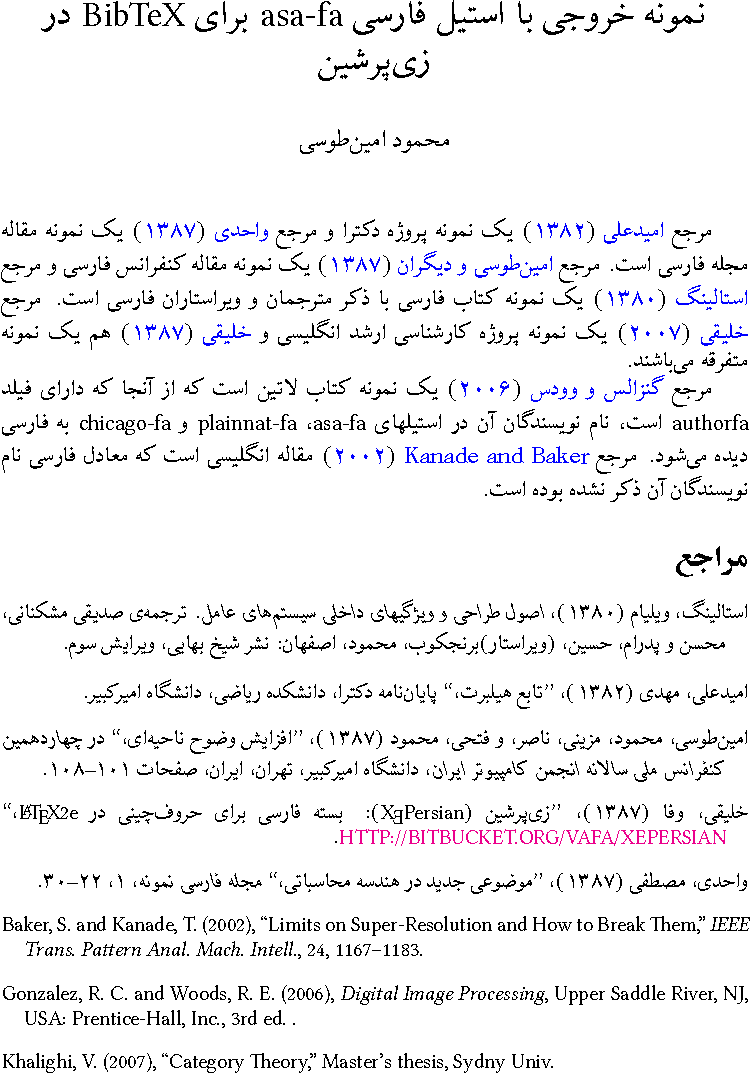
\includegraphics[width=.8\textwidth]{images/asa-fa-crop.pdf}
\caption{نمونه خروجی با سبک \lr{asa-fa}}
\label{fig:asafa}
\end{figure} 

\subsection{ نحوه استفاده از سبک‌های فارسی}


برای استفاده از بیب‌تک باید مراجع خود را در یک فایل با پسوند \lr{bib} ذخیره نمایید. یک فایل \lr{bib} در واقع یک پایگاه داده از مراجع\LTRfootnote{Bibliography Database}  شماست که هر مرجع در آن به عنوان یک رکورد از این پایگاه داده
با قالبی خاص ذخیره می‌شود. به هر رکورد یک مدخل\LTRfootnote{Entry} گفته می‌شود. یک نمونه مدخل برای معرفی کتاب \lr{Digital Image Processing} در ادامه آمده است:

\singlespacing
\begin{LTR}
\begin{verbatim}
@BOOK{Gonzalez02image,
  AUTHOR =      {Rafael Gonzalez and Richard Woods},
  TITLE =       {Digital Image Processing},
  PUBLISHER =   {Prentice-Hall, Inc.},
  YEAR =        {2006},
  EDITION =     {3rd},
  ADDRESS =     {Upper Saddle River, NJ, USA}
}
\end{verbatim}
\end{LTR}
\doublespacing

در مثال فوق، \lr{@BOOK} مشخصه‌ی شروع یک مدخل مربوط به یک کتاب و \lr{Gonzalez02book} برچسبی است که به این مرجع منتسب شده است.
 این برچسب بایستی یکتا باشد. برای آنکه فرد به راحتی بتواند برچسب مراجع خود را به خاطر بسپارد و حتی‌الامکان برچسب‌ها متفاوت با هم باشند معمولاً از قوانین خاصی به این منظور استفاده می‌شود. یک قانون می‌تواند فامیل نویسنده‌ی اول+دورقم سال نشر+اولین کلمه‌ی عنوان اثر باشد. به \lr{AUTHOR} و $\dots$ و \lr{ADDRESS} فیلدهای این مدخل گفته می‌شود؛ که هر یک با مقادیر مربوط به مرجع مقدار گرفته‌اند. ترتیب فیلدها مهم نیست. 

انواع متنوعی از مدخل‌ها برای اقسام مختلف مراجع همچون کتاب، مقاله‌ی کنفرانس و مقاله‌ی ژورنال وجود دارد که برخی فیلدهای آنها با هم متفاوت است. 
نام فیلدها بیانگر نوع اطلاعات آن می‌باشد. مثالهای ذکر شده در فایل \lr{MyReferences.bib} کمک خوبی به شما خواهد بود. 
%این فایل یک فایل متنی بوده و با ویرایشگرهای معمول همچون \lr{Notepad++} قابل ویرایش می‌باشد. برنامه‌هایی همچون 
%\lr{TeXMaker}
% امکاناتی برای نوشتن این مدخل‌ها دارند و به صورت خودکار فیلدهای مربوطه را در فایل \lr{bib}  شما قرار می‌دهند.  
با استفاده از سبک‌های فارسی آماده شده، محتویات هر فیلد می‌تواند به فارسی نوشته شود، ترتیب مراجع و نحوه‌ی چینش فیلدهای هر مرجع را سبک مورد استفاده  مشخص خواهد کرد.

نکته: بدون اعمال تنظیمات موردنیاز \lr{Bib\TeX} در \lr{TeXWorks}، مراجع فارسی در استیل‌هایی که مراجع را به صورت مرتب شده چاپ می‌کنند، ترتیب کاملاً درستی نخواهند داشت. برای توضیحات بیشتر \cite{persianbib87userguide} را ببینید. تنظیمات موردنیاز در \lr{TeXstudio} اعمال شده‌اند.

\textbf{برای درج مراجع خود لازم نیست نگران موارد فوق باشید. در فایل 
\lr{MyReferences.bib}
 که همراه با این \پ هست، موارد مختلفی درج شده است و کافیست مراجع خود را جایگزین موارد مندرج در آن نمایید.
}

پس از قرار دادن مراجع خود، یک بار \lr{XeLaTeX} را روی سند خود اجرا نمایید، سپس \lr{bibtex} و پس از آن دوبار \lr{XeLaTeX} را. در 
\lr{TeXstudio}
 کلید \lr{F8} و در \lr{TeXWorks} هم گزینه‌ی \lr{BibTeX} از منوی \lr{Typeset}، \lr{BibTeX} را روی سند شما اجرا می‌کنند.

برای بسیاری از مقالات لاتین حتی لازم نیست که مدخل مربوط به آنرا خودتان بنویسید. با جستجوی نام مقاله + کلمه \lr{bibtex}  در اینترنت سایتهای بسیاری همچون \lr{ACM} و \lr{ScienceDirect} را خواهید یافت که مدخل \lr{bibtex} مربوط به مقاله شما را دارند و کافیست آنرا به انتهای فایل \lr{MyReferences} اضافه کنید.

از هر یک از سبکهای \lr{Persian-bib} می‌توانید استفاده کنید، البته اگر از سه استیل آخر استفاده می‌کنید و مایلید که مراجع شما شماره بخورند باید بسته \lr{natbib} را با گزینه \lr{numbers} فراخوانی نمایید.
		% پیوست اول: مدیریت مراجع در لاتک
% !TeX root=main.tex

\chapter{‌جدول، نمودار و الگوریتم در لاتک}\label{App:Latex:More}
\thispagestyle{empty}

در این بخش نمونه مثالهایی از جدول، نمودار و الگوریتم در لاتک را خواهیم دید.
\section{مدلهای حرکت دوبعدی}
بسیاری از اوقات حرکت بین دو تصویر از یک صحنه با یکی از مدلهای پارامتری ذکر شده در جدول 
\ref{tab:MotionModels}
 قابل مدل نمودن می‌باشد.  
\begin{table}[ht]
\caption{مدلهای تبدیل.}
\label{tab:MotionModels}
\centering
\onehalfspacing
\begin{tabular}{|r|c|l|r|}
\hline نام مدل & درجه آزادی & تبدیل مختصات & توضیح \\ 
\hline انتقالی & ۲ & $\begin{aligned} x'=x+t_x \\ y'=y+t_y \end{aligned}$  &  انتقال دوبعدی\\ 
\hline اقلیدسی & ۳ & $\begin{aligned} x'=xcos\theta - ysin\theta+t_x \\ y'=xsin\theta+ycos\theta+t_y \end{aligned}$  &  انتقالی+دوران \\ 
\hline مشابهت & ۴ & $\begin{aligned} x'=sxcos\theta - sysin\theta+t_x \\ y'=sxsin\theta+sycos\theta+t_y  \end{aligned}$  & اقلیدسی+تغییرمقیاس \\ 
\hline آفین & ۶ & $\begin{aligned} x'=a_{11}x+a_{12}y+t_x \\ y'=a_{21}x+a_{22}y+t_y \end{aligned}$  & مشابهت+اریب‌شدگی \\ 
\hline  پروجکتیو & ۸ & $\begin{aligned} x'&=(m_1x+m_2y+m_3)/D \\ y'&=(m_4x+m_5y+m_6)/D \\ D&=m_7x+m_8y+1 \end{aligned}$  & آفین+\lr{keystone+chirping} \\ 
\hline  شارنوری & $\infty $ & $\begin{aligned} x'=x+v_x(x,y) \\ y'=y+v_y(x,y) \end{aligned}$  &  حرکت آزاد\\ 
\hline 
\end{tabular} 
\end{table}

\section{ماتریس}

شناخته‌شده‌ترین روش تخمین ماتریس هوموگرافی الگوریتم تبدیل خطی مستقیم (\lr{DLT\LTRfootnote{Direct Linear Transform}}) است.  فرض کنید چهار زوج نقطهٔ متناظر در دو تصویر در دست هستند،  $\mathbf{x}_i\leftrightarrow\mathbf{x}'_i$   و تبدیل با رابطهٔ
  $\mathbf{x}'_i = H\mathbf{x}_i$
  نشان داده می‌شود که در آن:
\[\mathbf{x}'_i=(x'_i,y'_i,w'_i)^\top  \]
و
\[ H=\left[
\begin{array}{ccc}
h_1 & h_2 & h_3 \\ 
h_4 & h_5 & h_6 \\ 
h_7 & h_8 & h_9
\end{array} 
\right]\]
رابطه زیر را برای الگوریتم 
 \ref{alg:DLT} لازم دارم.
\begin{equation}\label{eq:DLT_Ah}
\left[
\begin{array}{ccc}
0^\top & -w'_i\mathbf{x}_i^\top & y'_i\mathbf{x}_i^\top \\ 
w'_i\mathbf{x}_i & 0^\top & -x'_i\mathbf{x}_i^\top \\ 
- y'_i\mathbf{x}_i^\top & x'_i\mathbf{x}_i^\top & 0^\top
\end{array} 
\right]
\left(
\begin{array}{c}
\mathbf{h}^1 \\ 
\mathbf{h}^2 \\ 
\mathbf{h}^3
\end{array} 
\right)=0
\end{equation}

\section{الگوریتم با دستورات فارسی}
با مفروضات فوق، الگوریتم \lr{DLT} به صورت نشان داده شده در الگوریتم 
\ref{alg:DLT}  خواهد بود.
\begin{algorithm}[t]
\onehalfspacing
\caption{الگوریتم \lr{DLT} برای تخمین ماتریس هوموگرافی.} \label{alg:DLT}
\begin{algorithmic}[1]
\REQUIRE $n\geq4$ زوج نقطهٔ متناظر در دو تصویر 
${\mathbf{x}_i\leftrightarrow\mathbf{x}'_i}$،\\
\ENSURE ماتریس هوموگرافی $H$ به نحوی‌که: 
$\mathbf{x}'_i = H \mathbf{x}_i$.
  \STATE برای هر زوج نقطهٔ متناظر
$\mathbf{x}_i\leftrightarrow\mathbf{x}'_i$ 
ماتریس $\mathbf{A}_i$ را با استفاده از رابطهٔ 
\eqref{eq:DLT_Ah} محاسبه کنید.
  \STATE ماتریس‌های ۹ ستونی  $\mathbf{A}_i$ را در قالب یک ماتریس $\mathbf{A}$ ۹ ستونی ترکیب کنید. 
  \STATE تجزیهٔ مقادیر منفرد \lr{(SVD)}  ماتریس $\mathbf{A}$ را بدست آورید. بردار واحد متناظر با کمترین مقدار منفرد جواب $\mathbf{h}$ خواهد بود.
  \STATE  ماتریس هوموگرافی $H$ با تغییر شکل $\mathbf{h}$ حاصل خواهد شد.
\end{algorithmic}
\end{algorithm}

\section{الگوریتم با دستورات لاتین}
الگوریتم \ref{alg:RANSAC} یک الگوریتم با دستورات لاتین است.

\begin{algorithm}[t]
\onehalfspacing
\caption{الگوریتم \lr{RANSAC} برای تخمین ماتریس هوموگرافی.} \label{alg:RANSAC}
\begin{latin}
\begin{algorithmic}[1]
\REQUIRE $n\geq4$ putative correspondences, number of estimations, $N$, distance threshold $T_{dist}$.\\
\ENSURE Set of inliers and Homography matrix $H$.
\FOR{$k = 1$ to $N$}
  \STATE Randomly choose 4 correspondence,
  \STATE Check whether these points are colinear, if so, redo the above step
  \STATE Compute the homography $H_{curr}$ by DLT algorithm from the 4 points pairs,
  \STATE $\ldots$ % الگوریتم کامل نیست
  \ENDFOR
  \STATE Refinement: re-estimate H from all the inliers using the DLT algorithm.
\end{algorithmic}
\end{latin}
\end{algorithm}

\section{نمودار}
لاتک بسته‌هایی با قابلیت‌های زیاد برای رسم انواع مختلف نمودارها دارد. مانند بسته‌های \lr{Tikz} و  \lr{PSTricks}. توضیح اینها فراتر از این پیوست کوچک است. راهنمای همه آنها در تک‌لایو هست. نمونه مثالهایی از بسته \lr{Tikz} را می‌توانید در \url{http://www.texample.net/tikz/examples/} ببینید.

\section{تصویر}
نمونه تصاویری در بخش قبل دیدیم. دو تصویر شیر کنار هم را هم در شکل \ref{fig:twolion} مشاهده می‌کنید.
\begin{figure}[t]
\centering 
\subfigure[شیر ۱]{ \label{fig:twolion:one}

\includegraphics[width=.3\textwidth]{images/lion}}
%\hspace{2mm}
\subfigure[شیر ۲]{ \label{fig:twolion:two}

\includegraphics[width=.3\textwidth]{images/lion}}
\caption{دو شیر}
\label{fig:twolion} %% label for entire figure
\end{figure}
% !TeX root=main.tex

\chapter{وارد کردن کدهای برنامه‌نویسی}\label{App:Programming Code}
\thispagestyle{empty}

در این بخش نمونه مثال‌هایی از ورود کدهای برنامه نویسی ارائه خواهد شد. برای این منظور می‌توان از دو محیط زیر استفاده کرد. محیط اول مربوط به بسته 
\verb|listings|
 است که در آن تنظیمات مربوط به زبان برنامه‌نویسی به عنوان یک قابلیت اضافه وجود دارد. محیط دوم مربوط به بسته 
 \verb|verbatim|
 است. برای کسب اطلاعات بیشتر در مورد این دو بسته راهنمای آن‌ها را ببینید.
 
 محیط اول: زبان برنامه نویسی 
 \verb|Matlab|
 % به جای کلمه Matlab می توان متناسب با زبان مورد نظر از R , Python, SAS, PHP, C++, SQL, Java و ... استفاده کرد
\begin{latin}
\begin{lstlisting}[language=Matlab]
n = normrnd([1 2 3;4 5 6],0.1,2,3)
\end{lstlisting}
\end{latin}

محیط دوم: زبان برنامه 
 \verb|R|
 
 \begin{latin}
 \begin{verbatim}
set.seed(99)
x <- rnorm(100)
plot(density(x))
\end{verbatim}
 \end{latin}



%\baselineskip=.75cm
%\onehalfspacing
%\chapter*{واژه‌نامه فارسی به انگلیسی}\markboth{واژه‌نامه فارسی به انگلیسی}{واژه‌نامه فارسی به انگلیسی}
\addcontentsline{toc}{chapter}{واژه‌نامه فارسی به انگلیسی}
\thispagestyle{empty}

\englishgloss{Probabilistic}{احتمالی}
\englishgloss{Valuation}{ارزیابی}
\englishgloss{Measure}{اندازه }
\englishgloss{Stably}{پایدار}
\englishgloss{Weak Topology}{توپولوژی ضعیف}
\englishgloss{Powerdomain}{دامنه‌توانی}
\englishgloss{Function Space}{فضای تابع}
\englishgloss{Semantic Domain}{دامنه معنایی}
\englishgloss{Program Fragment}{قطعه‌برنامه}
\englishgloss{Dcpo}{مجموعه جزئاً مرتب کامل جهت‌دار}
\englishgloss{Ordered}{مرتب}
%\chapter*{واژه‌نامه  انگلیسی به  فارسی}\markboth{واژه‌نامه  انگلیسی به  فارسی}{واژه‌نامه  انگلیسی به  فارسی}
\addcontentsline{toc}{chapter}{واژه‌نامه  انگلیسی به  فارسی}
\thispagestyle{empty}

\persiangloss{مجموعه جزئاً مرتب کامل جهت‌دار}{Dcpo}
\persiangloss{فضای تابع}{Function Space}
\persiangloss{اندازه }{Measure}
\persiangloss{مرتب}{Ordered}
\persiangloss{دامنه‌توانی}{Powerdomain}
\persiangloss{احتمالی}{Probabilistic}
\persiangloss{قطعه‌برنامه}{Program Fragment}
\persiangloss{دامنه معنایی}{Semantic Domain}
\persiangloss{پایدار}{Stably}
\persiangloss{ارزیابی}{Valuation}
\persiangloss{توپولوژی ضعیف}{Weak Topology}

% برای آموزش نحوه خروجی گرفتن از واژه نامه‌ها به لینک زیر مراجعه کنید
% https://tex.stackexchange.com/questions/448387/glossary-and-abbreviation-showing-problem-in-xepersianshown-in-blank-pages
\newpage
\markboth{واژه‌نامه فارسی به انگلیسی}{واژه‌نامه فارسی به انگلیسی}
\printglossary[type=persian,style=mylistFa]
\newpage
\markboth{واژه‌نامه انگلیسی به فارسی}{واژه‌نامه انگلیسی به فارسی}
\printglossary[type=english,style=mylistEn]

% فهرست مقاله‌های برگرفته از پارسا. اطلاعات مقاله ها را در فایل 
% MyReferences.bib
% .وارد کنید. اگر مقاله ای ندارید سه خط زیر را غیر فعال کنید
\newpage
\thispagestyle{empty}
\thispagestyle{empty}
\makeatletter 
\renewcommand\BR@b@bibitem[2][]{\BR@bibitem[#1]{#2}\BR@c@bibitem{#2}}           
\makeatother
\nobibliography*
%  ترتیب مراجع در خروجی بر اساس ترتیب وارد کردن آن‌ها است. 
\begin{publicationspage}
\begin{latin}
\noindent
\bibentry{Baker02limits}\\[0.5cm]
\bibentry{Amintoosi09precise}
\end{latin}
\end{publicationspage}

% بخش کارنامک برای دانش‌آموختگان مقطع دکتری اجباری و برای مقطع کارشناسی ارشد اختیاری است. در صورتی که دانشجوی مقطع دکتری نیستید و نمی‌خواهید کارنامک داشته باشید سه خط زیر را غیرفعال کنید.
\newpage
\thispagestyle{empty}
\vspace*{1.5cm}
\thispagestyle{empty}
\section*{کارنامک}
\vspace*{1cm}
امین روشنی دانش‌آموختۀ دکتری تخصصی (کارشناسی ارشد) رشته آمار از دانشگاه .... در گرایش ..... در سال 1396 است. او در سال 1391 كارشناسی ارشـد (كارشناسـی) خود را از دانشگاه ..... در رشتۀ .... گرایش ..... و كارشناسی (کاردانی) خود را در سال 1387 از دانشگاه ..... در رشتۀ .... دریافت كرد. زمينه‌های پژوهشی او .....، ..... و ..... است.
% برگ تایید هیئت داوران به انگلیسی
\davaranPageEN

% دستوراتی برای نمایه

%{\baselineskip=.6cm
%	\phantomsection
%	\addcontentsline{toc}{chapter}{نمایه}
%	\printindex}

%\include{enRights}
% !TeX root=main.tex
% در این فایل، عنوان پایان‌نامه، مشخصات خود و چکیده پایان‌نامه را به انگلیسی، وارد کنید.

%%%%%%%%%%%%%%%%%%%%%%%%%%%%%%%%%%%%
\baselineskip=.6cm
\begin{latin}
\latinuniversity{Razi University}
\latinfaculty{Faculty of Science\\[0.25cm] Department of Statistics}
\latinsubject{Statistics}
\latinfield{Mathematic}
\latintitle{Writing projects, thesis and dissertations using Razi-Thesis Class}
\firstlatinsupervisor{First Supervisor}
\secondlatinsupervisor{Second Supervisor}
\firstlatinadvisor{First Advisor}
\secondlatinadvisor{Second Advisor}
\latinname{Amin}
\latinsurname{Roshani}
\latinthesisdate{January 2022}

\en-abstract{
This thesis studies on writing projects, theses and dissertations using Razi-Thesis Class. It ...
}
\latinkeywords{Writing Thesis, Template, \LaTeX, \XePersian}
\latinfirstPage
\end{latin}

\label{LastPage}

\end{document}
